%%%%%%%%%%%%%%%%%%%%%%%%%%%%%%%%%%%%%%%%%%%%%%%%%%%%%%%%%%%%%%%%%%%
%
%     McMaster University Physics & Astronomy PhD Thesis Template
%
%     filename  = "thesis.tex",
%     date      = "03/24/2015",
%     authors   = "Rory Woods",
%     copyright = "Rory Woods",
%     address   = "Physics & Astronomy,
%                  ABB,
%                  McMaster University,
%                  Hamilton, ON,
%                  CANADA",
%     telephone = "905-525-9140 ext",
%     email     = "woodsrm@mcmaster.ca",
%
%%%%%%%%%%%%%%%%%%%%%%%%%%%%%%%%%%%%%%%%%%%%%%%%%%%%%%%%%%%%%%%%%%%

\documentclass[twoside,letterpaper,phd]{macthesis}

%%%%%%%%%%%%%%%%%%%%%%%%%%%%
% Packages                 %
%%%%%%%%%%%%%%%%%%%%%%%%%%%%
\usepackage{fancyhdr}
\pagestyle{fancy}
\usepackage{deluxetable}
\usepackage{natbib} % \citet,\citep
\usepackage{aastex_hack} % Taken from: http://casa.colorado.edu/~danforth/comp/tex/thesistex.html
\usepackage{rotating}

\usepackage{amsmath}
\usepackage{amssymb}
\usepackage{amsthm}
\usepackage{exscale}
\usepackage[mathscr]{eucal}
\usepackage{bm}
\usepackage{eqlist} % Makes for a nice list of symbols.

%Rory-specific - algorithm typesetting environment
%\usepackage{algorithm2e}
\usepackage{caption}
\usepackage{subcaption}

%\usepackage[final]{graphicx}

\usepackage{epigraph}
\usepackage{lettrine}
\usepackage{keyval}

\usepackage[dvipsnames]{color}
%\usepackage{times}
%\documentstyle[fancyhdr]
%\usepackage{tabular}
%\DeclareGraphicsExtensions{.pdf, .jpg}


\usepackage{multirow}

%%%%%%%%%%%%%%%%%%%%%%%%%%%%
% Setting for fncychap     %
%%%%%%%%%%%%%%%%%%%%%%%%%%%%
% Comment out or remove the next two lines and you will get
% the standard LaTeX chapter titles. We like these A LOT
% better.
\usepackage[Lenny]{fncychap}
\ChTitleVar{\Huge\sffamily\bfseries}


%%%%%%%%%%%%%%%%%%%%%%%%%%%%%%%%%%%%
% SPECIAL SYMBOLS AND NEW COMMANDS %
%%%%%%%%%%%%%%%%%%%%%%%%%%%%%%%%%%%%
%\input{SupplementaryMaterial/UserDefinedCommands}


%%%%%%%%%%%%%%%%%%%%%%%%%%%%%%%%%%%%%%%%%
% Renewed Float Parameters              %
% (Makes floats fit better on the page) %
%%%%%%%%%%%%%%%%%%%%%%%%%%%%%%%%%%%%%%%%%
\renewcommand{\floatpagefraction}{0.85}
\renewcommand{\topfraction}      {0.85}
\renewcommand{\bottomfraction}   {0.85}
\renewcommand{\textfraction}     {0.15}



% Alter some LaTeX defaults for better treatment of figures:
% See p.105 of "TeX Unbound" for suggested values.
% See pp. 199-200 of Lamport's "LaTeX" book for detail
%   General parameters, for ALL pages:
\renewcommand{\topfraction}{0.9}	% max fraction of floats at top
\renewcommand{\bottomfraction}{0.8}	% max fraction of floats at bottom
%   Parameters for TEXT pages (not float pages):
\setcounter{topnumber}{2}
\setcounter{bottomnumber}{2}
\setcounter{totalnumber}{4}     % 2 may work better
\setcounter{dbltopnumber}{2}    % for 2-column pages
\renewcommand{\dbltopfraction}{0.9}	% fit big float above 2-col. text
\renewcommand{\textfraction}{0.07}	% allow minimal text w. figs
%   Parameters for FLOAT pages (not text pages):
\renewcommand{\floatpagefraction}{0.7}	% require fuller float pages
% N.B.: floatpagefraction MUST be less than topfraction !!
\renewcommand{\dblfloatpagefraction}{0.7}	% require fuller float pages

% ----------------------------------------------------------- %

%%%%%%%%%%%%%%%%
% FRONT-MATTER %
%%%%%%%%%%%%%%%%
% Title
\title{Radiative Transfer in Galaxies}
% Author and Department
\author{Rory Woods}
\dept{Physics and Astronomy}
% the degree will be conferred on this date
\degreedate{August 2015}
\copyrightyear{2015}


\documenttype{Thesis}

% This will generally be The Graduate School, though you can
% put anything in here to suit your needs.
\submittedto{The Graduate School}


%%%%%%%%%%%%%%%%%%
% Signatory Page %
%%%%%%%%%%%%%%%%%%
% You can have up to 7 committee members, i.e., one advisor
% and up to 6 readers.
%
% Begin by specifying the number of readers.
\numberofreaders{3}


\advisor[Thesis Advisor]
        {Dr. James Wadsley}
        {Associate Professor, McMaster University}

\readerone[Committee Member]
        {Dr. Laura Parker}
        {Associate Professor, McMaster University}

\readertwo[Committee Member]
          {Dr. Christine Wilson}
          {Professor, McMaster University}

\readerthree[External]
          {Dr. ???}
          {Professor, Somewhere Else}

% If using \include statements instead of \input statements,
% and you only want a subset of the \include statements to be
% evaluated, then declare your \includeonly here

%\includeonly{file1.tex,file2.tex,...}



%%%%%%%%%%%%%%%%%
% THE BEGINNING %
%%%%%%%%%%%%%%%%%

\begin{document}
\parindent=0.5in

%\graphicspath{{Figure/}} define figure search path

%%%%%%%%%%%%%%%%%%%%%%%%
% Preliminary Material %
%%%%%%%%%%%%%%%%%%%%%%%%
% This command is needed to properly set up the frontmatter.
\frontmatter


%%%%%%%%%%%%%%%%%%%%%%%%%%%%%%%%%%%%%%%%%%%%%%%%%%%%%%%%%%%%%%
% IMPORTANT
%
% The following commands allow you to include all the
% frontmatter in your thesis. If you don't need one or more of
% these items, you can comment it out. Most of these items are
% actually required by the Grad School -- see the Thesis Guide
% for details regarding what is and what is not required for
% your particular degree.
%%%%%%%%%%%%%%%%%%%%%%%%%%%%%%%%%%%%%%%%%%%%%%%%%%%%%%%%%%%%%%
% !!! DO NOT CHANGE THE SEQUENCE OF THESE ITEMS !!!
%%%%%%%%%%%%%%%%%%%%%%%%%%%%%%%%%%%%%%%%%%%%%%%%%%%%%%%%%%%%%%

% Generates the signature page. This is not bound with your
% thesis.
%\macsigpage


% Generates the committee page -- this is bound with your
% thesis. If this is an baccalaureate honors thesis, then
% comment out this line.
%\maccommitteepage


% Generates the title page based on info you have provided
% above.
\mactitlepage


% Generate the descriptive note page: Short-title page
\descriptivenote{supplementary/DescriptiveNote}


% Generates the abstract. The argument should point to the
% file containing your abstract.
\thesisabstract{supplementary/Abstract}

% Generates the Epigraph/Dedication. The first argument should
% point to the file containing your Epigraph/Dedication and
% the second argument should be the title of this page.
\thesisdedication{supplementary/Dedication}{}

%\thesiscoauthorship{supplementary/Coauthorship}

\thesisacknowledgments{supplementary/Acknowledgments}

\thesisepigraph{supplementary/Epigraph}


% Generates the Table of Contents
\thesistableofcontents



% Generates the List of Figures
\thesislistoffigures



% Generates the List of Tables
\thesislistoftables



% Generates the List of Symbols. The argument should point to
% the file containing your List of Symbols.
%\thesislistofsymbols{supplementary/ListOfSymbols}

% Generates the Acknowledgments. The argument should point to
% the file containing your Acknowledgments.
%\thesisacknowledgments{supplementary/Acknowledgments}





%%%%%%%%%%%%%%%%%%%%%%%%%%%%%%%%%%%%%%%%%%%%%%%%%%%%%%
% This command is needed to get the main part of the %
% document going.                                    %
%%%%%%%%%%%%%%%%%%%%%%%%%%%%%%%%%%%%%%%%%%%%%%%%%%%%%%

%\thesisepigraph{supplementary/Epigraph}


\thesismainmatter

%%%%%%%%%%%%%%%%%%%%%%%%%%%%%%%%%%%%%%%%%%%%%%%%%%
% This is an AMS-LaTeX command to allow breaking %
% of displayed equations across pages. Note the  %
% closing the "}" just before the bibliography.  %
%%%%%%%%%%%%%%%%%%%%%%%%%%%%%%%%%%%%%%%%%%%%%%%%%%
\allowdisplaybreaks{
%
%%%%%%%%%%%%%%%%%%%%%%
% THE ACTUAL CONTENT %
%%%%%%%%%%%%%%%%%%%%%%
% Chapters
%\begin{singlespace}
\begin{doublespace}
\pagestyle{fancy}
\headheight 20pt
\lhead{Ph.D. Thesis --- R. Woods}
\rhead{McMaster - Physics \& Astronomy}
\chead{}
\lfoot{}
\cfoot{\thepage}
\rfoot{}
\renewcommand{\headrulewidth}{0.1pt}
\renewcommand{\footrulewidth}{0.1pt}

\chapter{Introduction}
\label{chap:intro} 
\thispagestyle{fancy} 

It doesn't take much to convince a physicist of the importance of photons - astrophysical objects ``speak'' in photons. As astronomers, we receive all of our information in the universe through photons. In order to understand the objects we observe, we must understand photons and the physical processes that tie them to matter. 

\section{The Role of Radiation in Astrophysics}
\label{sec:radinastro}

When considering galaxies, for example, many of the galaxy properties are determined by the stars inside of it and the gas and dust between those stars. The rate at which a galaxy forms stars is dependent on the state of the gas, which is largely dependent on the Interstellar Radiation Field (ISRF), which is in turn dependent on the surrounding stars. While gas can be heated by other sources than the ISRF such as gravitational heating, for the purpose of this thesis, we focus on the ISRF.

In order to form stars, gas must be at low temperatures and high densities. This means gas cooling must be high compared to heating due to the ISRF. Cooling rates depend on the species present in the gas and the processes that are removing energy. Important processes include line cooling, bremsstrahlung radiation, synchrotron radiation, thermal emission from dust grains, and thermal x-ray emission. Many of the photons emitted in the above fashion can also act to heat the gas if the gas temperature is lower than the energy associated with the incident photons. Other heating sources include stellar emission, photoelectric heating, and (although they're not photons), cosmic rays.

If photon energies are higher than the binding energy of electrons in gas or dust, then electrons can be freed. In the case of atoms, this causes (photo) ionization. In the case of dust, it causes the dust grains to become negatively charged and the freed electrons to be available for photoelectric heating. In the case of molecules, the molecule can be dissociated.

Photoionization is most common with the most abundant gas elements, Hydrogen. This requires photons more energetic than 13.6 ev corresponding to the Extreme Ultraviolet (EUV) part of the spectrum. Near massive O and B stars, which emit heavily in the UV, these photons cause large ionized regions of Hydrogen, or HII regions. However, because these photons are so readily absorbed, they are largely absent from regions further from stars. Photons at energies higher than 13.6 ev not only ionize the atoms, but impart kinetic energy to the ejected electrons, which in turn heats the gas to average temperatures of 25,000 K.

In neutral regions where no H-ionizing photons are present, ionization of other elements become important. Due to Carbon's high abundance, it becomes the dominant heating mechanism. The energy needed to ionize Carbon is 11.3 ev, so photons between 11.3 ev and 13.6 ev become an important source of heating. 

Below 11.3 ev, the Far Ultra Violet (FUV) spectrum becomes important. Photons in this part of the spectrum are typical of large B stars, and while they don't have enough energy to ionize Hydrogen, they do have enough to free electrons from dust and Polycyclic Aromatic Hydrocarbon (PAH) molecules and impart kinetic energy to the freed electron. This drives one of the most important heating mechanisms in Interstellar Medium (ISM), photoelectric heating.

At energies much lower than FUV, photons become a a less important factor to heating and tend to act more as cooling mechanisms. Emission in the Infrared (IR) is especially common for dust cooling due to blackbody radiation.

Further sources of heating can be found at higher energies in X-rays, which have large energies but low intensity. X-rays become an important heating mechanisms for warm, low density, neutral gas.

%\begin{itemize}
%\item ISM
%\begin{enumerate}
%  \item photoelectric (PE)
%  \item cosmic rays (CR)
%  \item Carbon I (CI)
%\end{enumerate}
%\item Warm Neutral Medium
%\begin{enumerate}
%  \item CR/PE
%  \item X-rays
%\end{enumerate}
%\item Molecular Clouds
%\begin{enumerate}
%\item Cosmic Rays
%\item Turbulence
%\item Dust + gas
%\end{enumerate}
%\end{itemize}

Even with this very limited overview of heating and cooling, it becomes abundantly clear how important radiation is in determining the state of astronomical material. If we are to simulate the Universe, then we must properly capture the behavior of radiative transfer.

%
%\begin{itemize}
%\item Introduce stellar systems -  radiation can provide pressure support, can cause ionization, dissociation, can heat the gas. Because gas properties tied to star formation rate, and stars are one of the primary targets of observation, it's important to know what's going on.
%\item Introduce cosmology (how in depth here?). Cosmology depends on knowing photon history and what cosmological factors affect photons. Introduce cosmic reionization, Universe expansion, SZ?, lensing?, CMB?
%\item Need to ability to track photoionization, photoheating across huge amounts of sources and their environments. Astrophysical radiation has both short and large scale effects that can't be ignored.
%\end{itemize}

%[abelnormanmadau has good cosmo-intro w/ references.]


%Introduction to the basics of cosmology
%·         properties in the context of computational radiative transfer
%
%·         important evends like re-ionization of the universe
%
%·         ionization fronts and large numbers of sources
%
%·         with a focus on the physics side of things
%
% 
%Astro relies on photons - language of the universe
%·         only way the universe can be observe
%
%·         needs to be understood to get an idea of how things are interacting
%
% 
%Look at cosmology and stellar systems where these things are really important. 
%·         In order to understand why the algorithm needs to function the way it does, need to understand cosmology to have relevant applications
%
%·         Need to develop a what to represent approximations to deal with the large length scales and large number of sources.


%First part - what is this document? What will be in it? What is the main thing I will be telling you about? [Move this after intro to astro stuff? I think so...].



\section{Overview}
\label{sec:overview}

Chapter \ref{chap:radtransfer} will go over the background of radiative transfer and the currently available codes that solve the radiative transfer problem. It will also motivate the need for a new code in a particular niche. Chapter \ref{chap:method} will introduce the new radiative transfer method that we have developed. Chapter \ref{chap:codetests} will demonstrate the strengths and weaknesses of the new algorithm through a variety of numerical and phyical tests. Chapter \ref{chap:galaxyformation} will show the results of using the algorithm on an isolated galaxy in the FUV band, and will also focus on future projects that the algorithm will be used for. Finally, chapter \ref{chap:conclusions} contains the conclusions of this thesis.

\pagestyle{fancy}
\headheight 20pt
\lhead{Ph.D. Thesis --- R. Woods}
\rhead{McMaster - Physics \& Astronomy}
\chead{}
\lfoot{}
\cfoot{\thepage}
\rfoot{}
\renewcommand{\headrulewidth}{0.1pt}
\renewcommand{\footrulewidth}{0.1pt}

\chapter{Radiative Transfer}
\label{chap:radtransfer}

\thispagestyle{fancy}


\section{The Radiative Transfer Problem}
\label{sec:rtformulation}

When considering the transfer of photons, we must consider the scale we are dealing with. At the individual photon level, propagation is described by classical electrodynamics. Once we get to larger scales, however, it is more useful to treat radiation in ``packets'' or as an energy flux.

Consider an infinitesimal patch of area, dA, normal to a direction $\hat{n}$. We consider an infinitesimal solid angle, $d\Omega$, and consider all rays passing through the area and within the solid angle (see figure \ref{fig:intensity}).

\begin{figure}
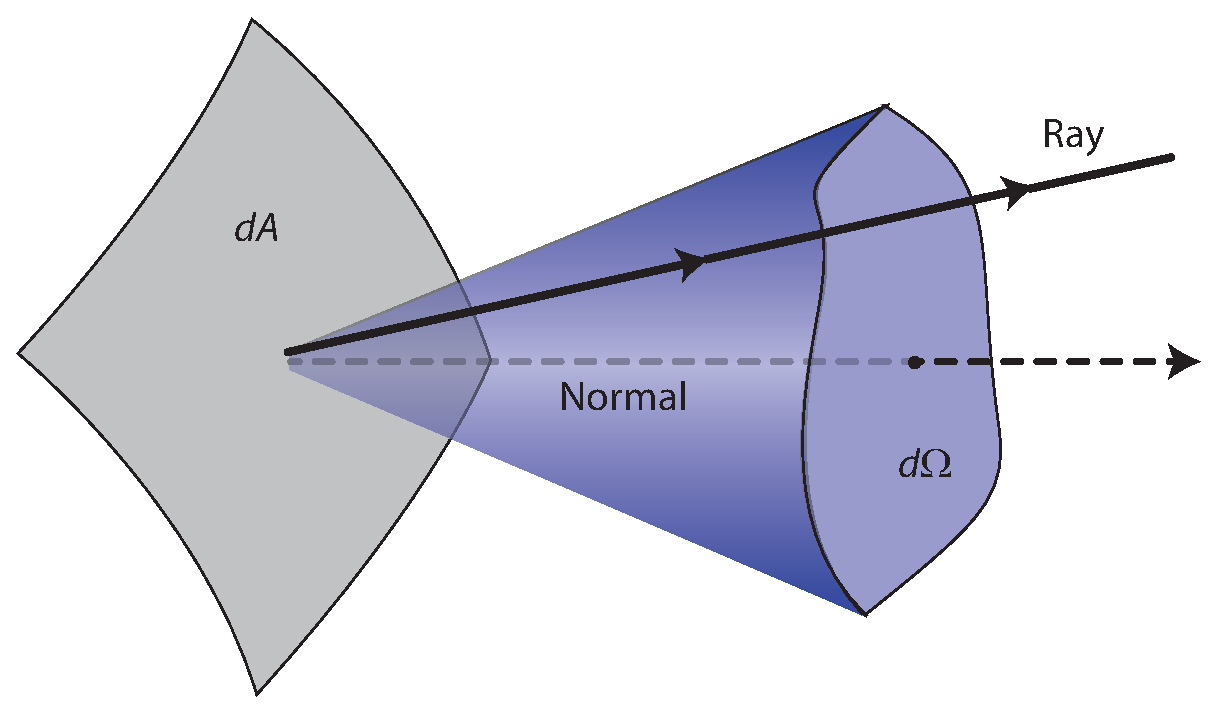
\includegraphics[width=\textwidth]{graphics/intensity.eps}
\caption[A visualization of how intensity is measured.]{The geometry for all rays at a point p through area dA within solid angle $d\Omega$. Figure adapted from \citet{rybickiLightman86}, figure 1.2.}
\label{fig:intensity}
\end{figure}

The energy through this area patch, within the solid angle, in time dt, and within the frequency range $d\nu$ is

\begin{equation}
\label{eq:intensity}
dE = I_{\nu}dA dt d\Omega d\nu,
\end{equation}

where $I_{\nu}$ is \emph{specific intensity} (specific because it is within a frequency range; dropping the frequency dependence makes this intensity). Specific intensity has units of energy per unit area per unit time per unit solid angle per unit frequency. It is useful to consider radiation in terms of intensity because it enables a macroscopic description of radiation that includes microscopic effects like scattering and absorption.

We can recover familiar values such as radiative flux, pressure, and density by taking moments of the intensity,

\begin{align}
\label{eq:moments}
E_{\nu} = \int I_{\nu}d\Omega,
F_{\nu} = \int I_{\nu}\cos{\theta}d\Omega,
P_{\nu} = \int I_{\nu}\cos{\theta}^2d\Omega,
\end{align}

where $E_{\nu}$ is the radiation energy density, $F_{\nu}$ is the specific flux (flux at a particular wavelength), and $P_{\nu}$ is the radiation pressure.

Let us now consider the passage of these rays through some matter. If we consider a ray, then energy may be added or removed from this ray due to absorption (removing photons), emission from the matter (adding photons), or scattering (scattering into or out of the ray). We first consider emission.

We define the specific (monochromatic) emission coefficient, j, as the energy emitted per unit time, per unit solid angle, per unit volume, and per unit frequency,

\begin{equation}
\label{eq:emissioncoef}
dE = j_{\nu} dV dt d\Omega d\nu.
\end{equation}

If we trace along a ray with cross section dA some distance ds, it will cover a cylindrical volume of $dV = dA ds$. Since equation \ref{eq:emissioncoef} and equation \ref{eq:intensity} only differ by a factor of distance (dA compared to dV), we can find the change intensity along the beam due to emission as

\begin{equation}
\label{eq:emissionintensity}
dI = j_{\nu} ds.
\end{equation}

Equation \ref{eq:emissionintensity} describes the amount of intensity added to a ray along some path ds due to spontaneous emission. If emission were the only process to worry about, finding intensity would be a simple matter of integrating the equation.

We next consider absorption. Consider again a ray traveling along a path ds. The amount of intensity lost due to absorption can be defined as

\begin{equation}
\label{eq:absorption}
dI = -\alpha I ds,
\end{equation}

where $\alpha$ is called the absorption coefficient and has units of distance$^{-1}$. It can be shown \citep{rybickiLightman86} that $\alpha$ is a function of more commonly known variables,

\begin{equation}
\label{eq:absorptioncoeff}
\alpha = -n \sigma I ds = -\rho \kappa I ds
\end{equation}

where n is the number density of particles, $\sigma$ is the cross section (in units of distance squared) of each absorbing particle, $\rho$ is the mass density, and $\kappa$ is the opacity (in units of distance squared per unit mass). Notice that the only difference between $n \sigma$ and $\rho \kappa$ is the average mass of the absorbing particles. We proceed from here using $\rho$ and $\kappa$, as these values are more directly available in our code.

Finally, we consider scattering. Scattering is a process that both subtracts and adds to the intensity. We can define a specific emission coefficient for scattering by equating the power per unit volume per frequency emitted to the power received,

\begin{equation}
\label{eq:scatteringcoefficient}
j_{s,\nu} = \sigma_{\nu} J_{\nu},
\end{equation}

where $\sigma_{\nu}$ is the specific scattering coefficient, and $J_{\nu}$ is the specific mean intensity, defined as

\begin{equation}
\label{eq:meanintensity}
J_{\nu} = \frac{1}{4\pi}\int I_{\nu} d\Omega.
\end{equation}

Before combining all of the processes affecting radiative transfer, it is useful to introduce a variable called the specific \emph{Source Function},

%\begin{align}
%S_{a,\nu} &\equiv \frac{j_{\nu}}{\alpha_{\nu}}, \label{eq:sourcefunction_a}\\
%S_{s,\nu} &\equiv \frac{j_{\nu}}{\alpha_{\nu}}. \label{eq:sourcefunction_s}
%\end{align}

\begin{equation}
\label{eq:sourcefunction}
S_{\nu} &\equiv \frac{j_{\nu}}{\alpha_{\nu}}.
\end{equation}


The source function is the ratio of emission to absorption and describes the intensity that an object will tend to. In the case of pure absorption, emission is 0 and so the source function is 0, since the intensity would tend to 0. In the case of pure emission, the source function is infinite and intensity tends to infinity since nothing is removing photons.

We now have the base equations to put together a description of radiative transfer that includes the processes of spontaneous emission, absorption, and scattering. Combining equations \ref{eq:emissionintensity}, \ref{eq:absorption}, \ref{eq:scatteringcoefficient}, \ref{eq:meanintensity}, and \ref{eq:sourcefunction}, we can write

\begin{align}
\label{eq:combinedtransfer}
\frac{dI_{\nu}}{ds} &= (-\alpha_{\nu}I_{\nu} + j_{\nu}) - (\sigma_{\nu}I_{\nu} + j_{s,\nu}) \nonumber\\
 &= -\alpha_{\nu}(I_{\nu} - S_{a,\nu}) - \sigma_{\nu}(I_{\nu} - J_{\nu}) \nonumber\\
 &= -(\alpha_{\nu} + \sigma_{\nu})(I_{\nu}-S_{\nu}),
\end{align}

where the combined source function $S_{\nu}$ is defined as

\begin{equation}
\label{eq:combinedsourcefunction}
S_{\nu} \equiv \frac{\alpha_{\nu}S_{a,\nu} + \sigma_{\nu}J_{\nu}}{\alpha_{\nu} + \sigma_{\nu}}.
\end{equation}

The above equation is an integro-differential equation - it is a function of $I_{\nu}$, $\frac{dI_{\nu}}{ds}$, and $\int I_{\nu} d\Omega$. Thus, any equation involving scattering is significantly more difficult to solve. Numerical solutions to integro-differential equations are usually specialized and complex [cite someone], and in the above case, the integral depends on all directions, making it especially costly.

For this reason, scattering is often omitted from radiative transfer solvers due to the very large added computational cost. In this thesis, our solutions do not explicitly account for scattering, though as is discussed in chapter \ref{chap:conclusions}, it is possible to add that functionality.

If scattering is omitted, equation \ref{eq:combinedtransfer} is simplified to a nicer form. We combine equations \ref{eq:emissionintensity}, \ref{eq:absorption}, and \ref{eq:sourcefunction_a} to obtain

\begin{equation}
\label{eq:transferequation_s}
\frac{dI_{\nu}}{ds} = -\alpha_{\nu}I_{\nu} + j_{\nu}.
\end{equation}

It is now useful to introduce optical depth $\tau_{\nu}$,

\begin{equation}
\label{eq:opticaldepth}
\tau(s) = \int_{s_0}^{s} \alpha_{\nu}(s')ds' = \int_{s_0}^{s} \rho(s') \kappa_{\nu}(s') ds'.
\end{equation}

Optical depth is a unitless value that describes the mean free path of a photon between interactions. The distance needed in the integral to give $\tau_{\nu} = 1$ should correspond to one mean free path given the absorption coefficient $\alpha_{\nu}$. It is useful to rewrite equation \ref{eq:transferequation_s} in terms of $\tau_{\nu}$ and $S_{\nu}$ by simply dividing by $\alpha_{\nu}$

\begin{equation}
\label{eq:transferequation_t}
\frac{dI_{\nu}}{d\tau_{\nu}} = -I_{\nu} + S_{\nu}.
\end{equation}

Equation \ref{eq:transferequation_t} is the transfer equation for radiation as it is most commonly seen. A solution can be obtained by using an integrating factor of $e^{\tau_{\nu}}$, which gives the formal solution to the transfer equation

\begin{equation}
\label{eq:transferequationsolution}
I_{\nu}(\tau_{\nu}) = I_{\nu}(0)e^{-\tau_{\nu}} + \int_0^{\tau_{\nu}} e^{-(\tau_\nu - \tau'_{\nu})} S_{\nu}(\tau'_{\nu})d\tau'_{\nu}.
\end{equation}

Solving the above equation at a point in a simulation would give you a radiation field that accounted for emission and absorption at all other points in the simulation. This would then be repeated at all points for which a radiation field is needed.

It is useful also to consider the case of only absorption. In many astrophysical simulations, only a single or few sources are modeled, and so the emission coefficient is zero at most points. For this reason, it become more efficient to just sum over all sources and treat only absorption. In this case, equation \ref{eq:transferequation_t} simplifies to

\begin{equation}
\label{eq:transferequation_abs}
\frac{dI_{\nu}}{d\tau_{\nu}} = -I_{\nu},
\end{equation}

which has the solution

\begin{equation}
\label{eq:absorptionsolution}
I_{\nu}(\tau_{\nu}) = I_{\nu}(0)e^{-\tau_{\nu}}.
\end{equation}

This creates a much simpler (though still quite difficult) problem to solve.

It should now be clear why radiative transfer is a difficult problem; analytically, it involves integrals over source functions that are not necessarily known at all points in space, with both density and opacity varying as a function of position as well. Numerically, we are trying to solve a function of seven variables - three position, two angular, time, and frequency - $I = I(x,y,z,\theta,\phi,t,\nu)$.

%\begin{equation}
%\label{eq:rademission}
%I(s) = I(s_0) + \int_{s_0}^{s} j(s') ds'
%\end{equation}
%
%\begin{equation}
%\label{eq:radabsorption}
%I(s) = I(s_0)\exp{\left[-\int_{s_0}^{s} \alpha(s') ds'\right]} = I(s_0)\exp{\left[ -\tau (s) \right]}
%\end{equation}

\section{Current Methods}
\label{sec:currentmethods}

The equations presented in section \ref{sec:rtformulation} are very difficult to solve if approximations are not made. Seven dimensions means that even if each dimension only has a resolution of 100 elements, we must keep track of $10^{14}$ elements, or roughly one petabyte of data if each element is just 10 bytes. In many cases, 100 elements is not nearly fine enough to resolve important features in a dimension, especially in frequency where many sharp features are present. The problem is already numerically impractical from a memory perspective.

As well, the full transfer equation is an integro-differential equation, meaning that common numerical solvers are not useful. Solvers for this type of equation are generally complex and specific purpose, so the actual numerical method side is also difficult.

In order to overcome the above, different approximations to the equation are adopted. Different approximations give rise to different advantages and disadvantages in accuracy and speed and typically apply best to particular regimes.

Current popular strategies include monte-carlo, ray tracing, moment methods, and a variety of others. The following sections will give a brief description of some of the most common and successful techniques as well as common properties of each method.

\subsection{Monte-Carlo Solvers}
\label{sec:montecarlo}

Monte-Carlo (MC) methods are perhaps the most obvious way to solve the radiative transfer problem. The most basic solution follows a photon from emission, through any scattering, absorption, and re-emission, until it leaves the simulation. At any point during the path, random numbers are used to determine whether the photon will be scattered, what direction it will be scattered, whether it will be absorbed, and what wavelength the re-emitted photon(s) will be.

Of course, following individual photons is not practical. Instead, following ``photon packets'' is more useful. Like intensity, packets are typically defined as having a specified energy (in which case, the number of photons can be determined by using $E = h\nu$ \citep{ercolanoEt03,abbottLucy85}.

In order to determine when a photon packet will interact, most codes use one of two methods. The first strategy is to use a probability distribution function (PDF) for optical depth. The PDF takes the form

\begin{equation}
\label{eq:taupdf}
P(l) = \frac{\int_0^{\tau(l)}e^{\tau}d\tau}{\int_0^{\infty}e^{\tau}d\tau} = 1-e^{-\tau},
\end{equation}

where P(l) is the probability of an interaction happening at a distance l and $\tau(l)$ is the optical depth corresponding to the interaction. By inverting equation \ref{eq:taupdf}, one can use a random number for P(l) to determine the interaction optical depth (or distance). The photon packet is then assumed to interact at that position, and the process is repeated \citep{harriesHowarth97}.

Another strategy is to simply trace the photon packet from resolution element to resoultion element (cells, particles), and at each point, to use a random number to determine if the photon packet should interact at that cell. This has the advantage that the code does not need to calculate and normalize optical depths \citep{lucy99,ercolanoEt03}.

The above process is repeated until a photon packet leaves the simulation volume, and is performed for many photon packets. Once a large number of photon packets have been sent out, physical quantities must be estimated from observed MC quantities. In this case, a common physical quantity to determine is mean intensity $J$ and the MC quantity is the photon packet. In order to relate the quantities, an \emph{estimator} is needed. An obvious choice (though not necessarily the most optimal \citep{ercolanoEt03}) is to simply use the definition of intensity (equation \ref{eq:intensity}),

\begin{equation}
\label{eq:mcstimator}
\Delta E = I_{\nu}(r,\theta)\Delta A |\cos{\theta}|\Delta \nu \Delta \omega \Delta t,
\end{equation}

Where $\Delta A$ is the reference surface, $\theta$ is the angle between the photon packet vector and surface normal vector, $\Delta \omega$ is the solid angle, $\Delta \nu$ is the frequency range, and $\Delta t$ is the time interval. By combining with equation \ref{eq:meanintensity}, one can obtain a mean intensity from a sum of photon packets \citep{ercolanoEt03},

\begin{equation}
\label{eq:mcmeanintensity}
J_{\nu}(r) = \frac{1}{4\pi}\frac{\Delta E}{\Delta t} \sum_i^{N_k} \frac{1}{\cos{\theta}}\frac{1}{\Delta A}\frac{1}{\Delta \nu}.
\end{equation}

Once a mean intensity is found at a location, a solution for ionization can be iterated to by integrating out the ionization and heating terms with the mean intensity. Note that it must be iterated since a change in ionization and temperature may imply a change in local absorption properties.

The MC process is very accurate. It can deal with arbitrary spatial distributions, arbitrary scattering functions, polarization, and provides a natural way for ``observing'' a simulated object.

However, MC is \emph{very} computationally costly. Large numbers of photon packets must be sent out and individually tracked in order to get a good estimate of the true mean intensity. Due to the random nature, typically errors only converge as 1/$\sqrt{N_{\gamma}}$, where $\sqrt{N_{\gamma}}$ is the number of photon packets per source. While photons can be added to a packet along its path by gas and dust, new photon packets must be created for all stellar sources to guarantee their emission is added. This means as more sources are added, the computational cost rises linearly.

There is also an indirect cost associated with optical depth. In the case of very optically thick systems, interactions occur far more often between photon packets and the medium, meaning more computation is needed per photon packet. In the case of very optically thin systems, interactions are very rare and very large numbers of photons must be cast to get accurate statistics on heating, ionization, and scattering. 

From a numerical perspective, MC provides poor error control. Higher accuracy requires an increase in the number of photons. However, as was mentioned, this converges very slowly and often still does not guarantee good statistics on rare events such as low probability re-emission or scattering.

For the above reasons, MC radiative transfer is most commonly used as a post-processing technique for creating images of astrophysical objects. For more details on specific codes, please see \citet{dullemond12,cantalupoPorciani11,altayEt08,ercolanoEt03,nenkovaEt99,lucy99,harriesHowarth97}, among many others.

%In monte-carlo methods, a photon is carefully tracked through a domain, following scattering, absorption, and re-emission. See [from steinacker 09] \citet{wolf03,woodEt2004,ercolanoEt2005,jonsson06,pinteEt06}.

%\begin{itemize}
%\item Advantages - can treat complicated spatial distributions, arbitrary scattering functions, and polarization.
%\item Disadvantages - Very high or low optical depths hard (why?), re-emission in all directions over many events hard (why?), no global error control
%\end{itemize}


\subsection{Ray Tracing}
\label{sec:raytracing}

At the most basic level, Ray Tracing is a fairly natural way to go about solving the equations of radiative transfer and is probably the most popular method in astrophysics. Rays are cast from sources and the energy or photons contained in the ray are diminished as it passes through absorbing material \citep{altayTheuns13, razoumovScott99,abelNormanMadau99}. This may sound familiar to section \ref{sec:montecarlo} because many Monte Carlo codes often use a ray tracing approach to follow their photon packets.

Most ray tracing codes tend to start by simplifying the radiative transport equation (\ref{eq:transferequation_s}) by assuming the the emissivity of intervening material is 0. This leads to a much simplified version of the equation

\begin{equation}
\label{eq:transferequation_abs}
\frac{dI_{\nu}}{d\tau_{\nu}} = -I_{\nu},
\end{equation}

which has the simple solution

\begin{equation}
\label{eq:transfersolution_abs}
I_{\nu} = I_{\nu}(0)e^{-\tau_{\nu}}.
\end{equation}

It remains only for the ray tracer to calculate the optical depth between a source and another point. The simplest strategy to do this is to send rays out that intersect every cell in the simulation, and simply remove photons from the ray as they pass through each cell according to equations \ref{eq:opticaldepth} and \ref{eq:transfersolution_abs}. This process is visualized in figure \ref{fig:raytracing}.

\begin{figure}
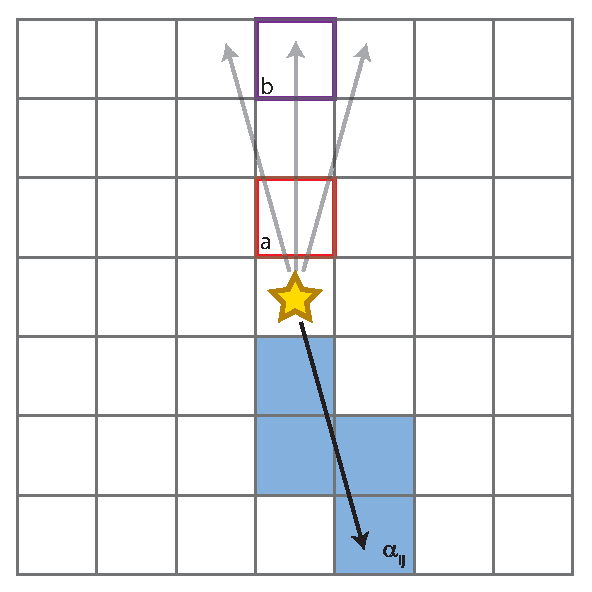
\includegraphics[width=\textwidth]{graphics/ray_flux.eps}
\caption[A visualization of ray tracing.]{Rays being traced through a grid in a simulation. Each ray has an associated energy or number of photons that are removed from the ray as it traverses through each cell according to the properties of each cell. The blue highlighted cells show an example for one particular ray, where intensity is removed according to the absorption coefficient, $\alpha_{i,j}$, of each cell it passes through. Notice that closer cells, such as cell a, have more rays intersecting them than further cells, such as cell b, meaning redundant work is performed in the close cells.}
\label{fig:raytracing}
\end{figure}

In principle, this process would solve the radiative transfer problem provided enough rays were cast. However, many practical problems arise that require special care. When casting rays, closer cells are intersected by far more rays than far away cells, as can be seen in figure \ref{fig:raytracing}, comparing cells a and b. This means redundant work is performed near the source in order to get sufficient resolution of intensity at large distances. Many codes have created adaptive techniques to reduce the number of rays that are needed. For example, \citet{abelWandelt02} make use of the HEALPIX algorithm \citep{gorskiEt99} to determine rays that create an equal area per ray on a sphere. As the ray moves out and the ratio of the surface area of a cell to the solid angle of a ray decreases, the HEALPIX algorithm is recursively called on a single ray to subdivide it into four smaller rays to better sample further cells. This reduces the number of rays that need to be cast (see figure 2 in \citet{abelWandelt02}).

A more difficult problem that arises is the computational cost associate with more sources. For most ray tracing codes, every additional source requires the whole tracing procedure to be performed again. While there are a few codes that have attempted to remove this poor scaling [fill in authors], it is more often seen as a limitation of the method and so the method is not often applied to problems with large numbers of sources [I don't know if I like this sentence].

While the above description was based off of the initial assumption that scattering was zero, ray tracing codes do exist that attempt to model scattering in some way. Some authors have chosen to break the field into a direct component (due to ionizing sources) and a diffuse component (due to recombination in gas). The diffuse component can then be tracked and solved separately from the direct component. For example, \citet{razoumovScott99} chooses to use an operator split explicit-implicit scheme to advect the radiation variable along the separate rays. Other authors, e.g. \citet{abelNormanMadau99}, use a similar approach advecting the diffuse radiation, but choose not to keep track of rays at this point.

The scenarios presented up until now have all focused on sending rays out from sources. URCHIN \citep{altayTheuns13} is a ray tracing code that has adopted the opposite strategy of sending rays out from sinks. While this may seem counter-intuitive at first, there are many computational advantages to doing this in particular physical scenarios. \citet{altayTheuns13} designed the algorithm to efficiently model the post-reionization Universe, where radiation is coming from all directions. In this case, tracing rays outward from sinks is guaranteed to find sources of radiation and alleviates any sampling issues associated with choosing sources to start tracing from.

Note that many of the algorithms mentioned above rely on tracing radiation outward along structured data. If the data is unstructured, it is far more difficult to properly estimate what portion of ray segments are affected by absorbing media. As well, it becomes very difficult to ensure that sufficiently many rays are propagated to each resolution element. Unfortunately, this is exactly the scenario that is present in SPH simulations, where resolution elements are completely irregular.

\citet{pawlikSchaye} have created a short-characteristics ray tracing scheme specifically designed to deal with the unstructured nature of SPH simulations called TRAPHIC. In this ray tracer, radiation is ``traced'' out in cones to neighboring SPH particles. However, since particles do no necessary exist in all directions for a given particle, virtual particles can be introduced to help propagate radiation through voids without particles. Note that by keeping a fixed solid angle for each particle, a natural adaptivity arises since the same solid angle on a particle further from a source will cover a smaller solid angle with respect to the source. TRAPHIC also introduces a method of merging sources that are close in angle for a receiving gas particles. Merging sources means that the algorithm can handle very large numbers of sources, making it one of the most currently powerful algorithms for cosmological simulations. [transition...]

The ray tracing method affords many advantages - it can handle arbitrary geometries and gives good error control, meaning very accurate results can be obtained. However, the method is typically limited to simulations that contain small numbers of sources due to poor scaling. As well, the method tends to have difficulty with very high optical depths and it usually becomes more practical to use a moment method (section \ref{sec:momentmethods}) [why is this? is this because of time steps? Says more complicated solvers needed? Mention time steps...].


%ray tracing need 4piR^2/deltax^2 rays to sample far away cells, gives inner sampling of (r/R)^2, wasteful.
%Ray tracing has the ability to treat arbitrary density distributions, and can use general solvers for ODEs. Fairly accurate and fairly expensive.
%
%\begin{itemize}
%\item Often combined with monte-carlo methods
%\item Provides quite accurate results.
%\item Provides global error control.
%\item Can cause step-size limitations in order to consistently transfer photons.
%\item Becomes impractical at high optical depth and can require complicated solvers.
%\end{itemize}

%razoumovScott99 - account for travel time in similar way I suggested.

\subsection{Moment Methods}
\label{sec:momentmethods}

[Add citations to OTVET, description of., davis et al? short vs long characteristic.]

Moment methods represent a large chunk of astrophysical radiative transfer codes currently available. Very broadly, these methods take moments of the radiative transfer equations and make simplifications to make the equations easier to solve by common techniques.

Specifically, we can start by taking angular moments of the radiative transfer equation (equation \ref{eq:transferequation_t}?). If this is done in a frame comoving with the radiating fluid and local thermodynamic equilibrium is assumed, we get (to first order in v/c) \citep{mihalasMihalas84}

\begin{align}
&\frac{D\rho}{Dt} + \rho \mathbf{\nabla \cdot v} = 0,\label{eq:rhd1}\\
&\rho \frac{D\mathbf{v}}{Dt} = -\nabla P + \frac{1}{c}\chi_F \mathbf{F},\label{eq:rhd2}\\
&\rho \frac{D}{Dt}\left(\frac{E}{\rho}\right) = -\mathbf{\nabla \cdot F} - \mathbf{\nabla v:P} + 4\pi\kappa_p B - c\kappa_E E,\label{eq:rhd3}\\
&\rho \frac{D}{Dt}\left(\frac{e}{\rho}\right) = -P\mathbf{\nabla \cdot v} - 4\pi \kappa_P B + c\kappa_E E,\label{eq:rhd4}\\
&\frac{\rho}{c^2}\frac{D}{Dt}\left(\frac{\mathbf{F}}{\rho}\right) = -\mathbf{\nabla \cdot P} - \frac{1}{c} \chi_F \mathbf{F}.\label{eq:rhd5}
\end{align}

In the above equations, $D/Dt$ is the convective derivative, defined as $D/Dt \equiv \partial / \partial t + \mathbf{v}\cdot \nabla$. The quantities $\rho$, e, $\mathbf{v}$, and p are the mass density, energy density, velocity, and scalar isotropic pressure, respectively. E, $\mathbf{F}$, and $\mathbf{P}$ are the frequency-integrated radiation energy density, momentum density or flux, and pressure tensor, respectively. E, $\mathbf{F}$, and $\mathbf{P}$ are the zeroth, first, and second order angular moments of intensity (equation \ref{eq:intensity}),

\begin{equation}
A^n(\mathbf{x},t) = \oint I \cos^{n}{\theta}d\Omega.
\end{equation}

$\chi_F$ is the flux mean total opacity, $\kappa_P$ is the planck mean absorption opacity, and $\kappa_E$ is the energy mean absorption opacity. The first opacity represents an effective opacity with contributions from absorption and scattering across all wavelengths. [The second and third are absorption opacities....?]. Finally, c is the speed of light. [What is B? Planck? What is : in math equation?]

%\subsubsection{Flux Limited Diffusion}

%add whitehouse & bate
One popular moment method is Flux Limited Diffusion (FLD) \citep{almeWilson74,levermorePomraning81,pomraning83,meliaZylstra91,anileRomano92}. In FLD, the assumption is made that intensity is a slowly varying function of space and time. This is certainly true in the limit of very high or very low optical depth. It is the intermediate region ($\tau \approx 1$) where this assumption may not be true. This assumption allows the radiative flux to be written in the form of Fick's Law of diffusion \citep{levermorePomraning81},

\begin{equation}
\label{eq:fluxfdiffusion}
\mathbf{F} = -D\nabla E,
\end{equation}

where D is the diffusion coefficient, given by

\begin{equation}
\label{eq:diffusioncoeff}
D = \frac{c\lambda}{\chi}.
\end{equation}

$\lambda$ is a dimensionless function of energy called the flux limiter.

In order to solve equations \ref{eq:rhd1}-\ref{eq:rhd5}, the system must be closed by relating the moments of radiation. An obvious first choice is the Eddington Approximation, which assumes the field is isotropic and implies that

\begin{equation}
\label{eq:eddingtonapprox}
\mathbf{P} = \frac{1}{3}E.
\end{equation}

Using this approximation, equation \ref{eq:rhd5} becomes

\begin{equation}
\label{eq:eddingtonrhd}
\mathbf{F} = -\frac{c}{3\chi}\nabla E,
\end{equation}

which is correct in the optically thick limit, but gives an infinite speed of light in optically thin regions. Thus, the flux limiter in equation \ref{eq:diffusioncoeff} functions to allow the Eddington Approximation to be made by creating physical behavior in the optically thin regime by limiting the radiation propagation speed [reword].

By combining equations \ref{eq:fluxfdiffusion} and a relationship between moments of intensity, equations \ref{eq:rhd1}-\ref{eq:rhd4} can be solved numerically \citep{turnerStone01}.[Should I go into the actual solving process? I don't think so...]

Other common moment methods follow a similar path, but use different assumptions for the closure relation. Another popular choice is called the ``M1 closure relation'' \citep{levermore84, skinnerOstriker13}[add more codes here]. This assumes that intensity is rotationally invariant about the direction of radiative flux, rather than fully isotropic. This assumption allows better results in particular scenarios (e.g. shadowing behind dense objects \citep{skinnerOstriker13}) and a more efficient numerical solution \citep{gonzalezEt07,aubertTeyssier08}. However, its applications are limited as it cannot deal with complex radiation fields from distributed sources since it uses entirely local information to get the closure relation.

%add stone et al 92
The majority of moment methods tend to have a difficult time dealing with complex source distributions because they adopt a closure relation that only accounts for local characteristics of the radiation field. One moment code (among others) that has managed to get around this is OTVET \citep{gnedinAbel01}. OTVET explicitly constructs the radiation pressure tensor from the source distribution in the simulation, removing the need to assume a relationship between moments. This enables a combination of contributions to the intensity from all sources.

Overall, moment methods provide a useful and efficient way to solve problems that consist of high optical depth, where long characteristics are not important, or low optical depth with simple source distributions, so the intensity field is simple. Note that the method also tends to be very diffusive in many cases, and so special care must be taken to avoid this behavior if it is not desired.

\subsection{Other Methods}
\label{sec:othermethods}

Sections \ref{sec:montecarlo}-\ref{sec:momentmethods} cover some of the most common radiative transfer methods currently used in astrophysics. However, it is worth mentioning a few other methods that aren't as easily grouped into the above categories.

In order to overcome some of the shortcomings of moment methods and ray tracing methods, some authors have created hybrid codes that use both methods in different regimes in the simulation. \citet{kuiperEt10} has created one such scheme. The basic idea is to attempt to use each method in the regime where it's most advantageous to save on computation and improve accuracy. In the case of \citet{kuiperEt10}, the algorithm is designed to approach the problem of massive star formation. It uses a first order ray tracer to transfer stellar photons at higher frequencies to the gas. A secondary moment method (FLD) then diffuses the photons through high density gas. This is meant to efficiently model transfer of high frequency photons from a massive star and reprocessing of those photons to lower frequency emission.

The method avoids the difficulties that ray tracing can have in high optical depth regions and benefits from the speed and accuracy of FLD in appropriate physical regions. While the hybrid code of \citet{kuiperEt10} was specialized to do simulations of a single massive star, the code has since been extended to work on an arbitrary number of sources \citep{klassenEt2014}.

Another strategy is to make use of the Fast Fourier Transform (FFT) techniques. \citet{cen02} makes use of the property that if the sum of a quantity over a volume can be written in the standard convolution form, than it can be solved using an FFT. By re-writing equations \ref{eq:} and \ref{eq:} in this form, one can solve the equations in $N\log(N)$ time for each direction. Using trees to discretize the angles, you end up with roughly $\log(N)$ angles to solve for, and so the solution scales as $N\log^2(N)$. [More here.... I don't get this method.]

Finally, \citet{clarkEt12} have created an algorithm most similar to ray tracers, but whose purpose is to calculate column depths for exterior sources [check if this is right]. The basic idea is to map the simulation volume onto a sphere that has been divided into equal area segments by the HEALPIX algorithm \citep{gorski99}. By performing this action during the tree walk, columns can be calculated to any point within the simulation at a cost of $N\log(N)$. However, since this algorithm only calculates column depth as a function of $\theta, \phi$ for each particle, it is limited to cases in which sources are located outside of all absorbing material.

%Grid methods, statistic approach (MC?), fourier transforms (cen), hybrid methods (rijkhorst, mikhail), treeCOL, TRAPHIC.

%\subsection{Grid-Based Methods}
%\label{sec:gridmethods}
%
%Can use simple solvers (finite differencing or short characteristics) and gives good error control.
%
%\begin{itemize}
%\item Grid must be adaptable to be practical, though good refinement criteria is unclear
%\item Interpolation between grids can be costly and give interpolation errors.
%\item Numerical diffusion typically not taken into account.
%\end{itemize}

\section{Summary of Methods}
\label{sec:summaryofmethods}

Section \ref{sec:currentmethods} gave an overview of some of the most common methods currently used in astrophysics, so we are now well posed to assess the field of computational radiative transfer.

In order to solve the equations of radiative transfer, codes must make certain approximations. In all but MC codes, authors typically start by dropping scattering. Moment methods typically make a further assumption about the relationship between the moments of radiation, with the most common being the Eddington Approximation (eqation \ref{eq:eddingtonapprox}), or the assumption of radiation isotropy.

The above assumptions are still often not sufficient to make the problem computationally viable. Ray tracing has needed to make algorithm-specific improvements to become more computationally efficient. Making rays adaptive as they get further from the source reduces redundant work near the source, and in some scenarios, tracing the rays backwards from the sinks can provide another efficiency boost. Some codes, both ray tracing and moment methods, have also made the improvement of merging sources, which can reduce the number of sources to do calculations for from N to $\log(N)$.

Very roughly, the current code base occupies particular spaces in the computational radiative transfer volume. Monte carlo codes are typically the most accurate, but also the most computationally expensive. For this reason, they are usually limited to post processing and image creation in simulations. Ray tracers are the most popular, and offer very good accuracy, but typically scale quite poorly with the number of sources, and so are usually limited to simulations containing small numbers of sources. Moment codes are a step up in computational speed, but are usually only appropriate in simulations that have high optical depth where the assumption of radiation isotropy is appropriate. Otherwise, unwanted diffusion in the radiation field can give large errors. Despite the simplifying assumptions, many moment codes are still the dominant computational cost in simulations compared to other common physics solvers such as gravity and hydrodynamics.

Currently, there is a gap in the market for solvers that can deal with large numbers of sources over a range of optical depths without any diffusive assumptions. OTVET \citep{gnedinAbel01} is close to this regime, and perhaps the most widely recognized tool for cosmological simulations at the time, but is still a diffusive code [?]. TRAPHIC is currently the only code that satisfies the above criteria, and has recently started to take impressive steps forward on the computational cosmology front. TRAPHIC is SPH-specific, and so the algorithm is limited in this way. However, it is probably the most appropriate tool at the time for cosmological radiative transfer.

%\citep{pawlikEt15,jeonEt15,jeonEt14b,jeonEt14a,pawlikEt14,rahmatiEt13b,rahmatiEt13a,jeonEt12}

The goal of this thesis is to present a new algorithm for solving radiative transfer that is capable of dealing with large numbers of sources, non-diffusive, at a similar computational cost to gravity. In order to achieve these goals, we do not stress achieving exact solutions, but aim for correct qualitative behavior and correct equilibrium solutions.

\section{TO-DO (REMOVE THIS)}

\begin{itemize}
\item RAMSES-RT \citep{rosDahlTeyssier15,rosdahlEt13}
\item Mention error convergence
\end{itemize}


%The current set of computational methods can be classified as follows:
%
%\begin{itemize}
%\item Very accurate, expensive methods - monte carlo, ray tracing
%\item Methods accurate in specific scenarios, e.g. FLD for optically thick, ``str\"omgren method'' from Dale
%\item \emph{Very} rough approximations, e.g. method that only looks at absorption near sink and source.
%\end{itemize}
%
%As will be seen, there is currently an opening in the market for something in the middle - Decent accuracy at a low cost.


\pagestyle{fancy}
\headheight 20pt
\lhead{Ph.D. Thesis --- R. Woods}
\rhead{McMaster - Physics \& Astronomy}
\chead{}
\lfoot{}
\cfoot{\thepage}
\rfoot{}
\renewcommand{\headrulewidth}{0.1pt}
\renewcommand{\footrulewidth}{0.1pt}

\chapter{The Numerical Method}
\label{chap:method}
\thispagestyle{fancy}

In the absence of absorbing material, the problem of radiative transfer reduces down to that of gravity. As such, the tree-algorithm for calculating gravity can be used \citep{barnesHut86}.

\begin{itemize}
\item A tree can be used to partition space.
\item Each level of the tree holds finer partitions of the volume. See figure \ref{fig:tree}
\item Each node of the tree contains accumulated information about the tree below it (total mass, etc.).
\item In order to calculate gravity on a particular leaf (bucket), you can interact with the moment of another cell (\ref{eq:gravitymoment}).
\item To decide what level of the tree to interact with, you can define an opening angle/radius, $\theta$. If a cell is smaller than this opening angle (the distribution of matter inside the cell is contained within a small enough angle on the sky), the entire cell can be used in the force calculation. If not, you must consider the child nodes separately. See equation \ref{eq:openingangle}.
\item On average, the number of interactions a each particle will have is $\log{N}$, where N is the total number of particles. Thus, the force calculation for the whole simulation scales as $N\log{N}$. Note that lowering $\theta$ shifts the number of calculations that are approximated by large cells to smaller cells, and thus if $\theta$ is very small, the code approached scaling of order $N^2$.
\item In the case of radiation, the math is very similar (See eq \ref{eq:radiationmoments}). However, since radiation does not cancel like forces, the dipole moment does not disappear and a rougher approximation is possible (wording wrong, fix this).
\item In this case, the interaction scales as $N_{\mbox{sink}}\log{N_{\mbox{source}}}$. However, assuming the full tree is still used, the tree-build still scales as $N\log{N}$.
\end{itemize}

\section{Tree Data Structures}
\label{sec:treestruct}

In order to understand the radiative transfer algorithm that we are presenting, it is important to understand tree data structures.

\begin{itemize}
\item Terminology: Node, root node, leaf tree, interior node, child, parent, sibling, tree build, walk the tree, ascend the tree, descend the tree.
\item In computer science, a tree is a hierarchical data structure. Typically the tree starts at a single point, usually called the root node, and branches out to many other ``child'' nodes.
\item Each node in the tree stores some sort of data, and the relative location of the node in the tree indicates the relation of the data in the node to the data in other nodes.
\item \textsc{Gasoline} uses a ``k-d tree'' for gravity. This is an example of a binary space-partitioning tree. Every node contains 2 children, and each node of the tree represents a particular volume of space. kd-Trees and octrees represent the majority of trees used in astrophysical simulations.
\end{itemize}

\section{Building a Radiation Tree}
\label{sec:buildingtree}

\begin{itemize}
\item While the algorithm we present is general enough to work with any volume-filling tree, the following sections will introduce the algorithm as we have developed it. \textsc{Gasoline} uses a k-d tree for its gravity solver, and as such, our version of the algorithm stuck with this tree type in order to make use of existing tools in the code base.
\item The recursive pseudocode for the tree-build is presented below (note - change to nice pseudocode format):
	\begin{enumerate}
	\item if number of data elements greater than n$_{\mbox{leaf}}$, partition data
	\item recursively call build tree on each partition of the data set
	\item else, if number of data elements less than n$_{\mbox{leaf}}$, calculate basic cell properties
	\item After if statement, calculate accumulated cell properties (higher moments, etc)
	\end{enumerate}
\item In our case, the partition data step involves finding the longest axis of the data contained on the current node and dividing particles to the upper and lower halves of the midway point of that axis.
\item Each volume and its corresponding list of particles is then passed recursively to the tree build function again. This terminates when build tree receives a list of particles that is sufficiently short (less than a user set parameter, n$_{\mbox{leaf}}$). At this point, basic cell properties such as center of luminosity and total luminosity are calculated.
\item Once the leaf nodes have been calculated, more complicated average properties, such as higher moments, can be calculated by looping through all particles in the node. This applies to both leaf and interior nodes.
\item The initial partition function does not require that the data be fully sorted, only that it be divided to either side of an intermediate value. This is an order n operation.
\item The tree will be roughly of depth $\log(N)$, meaning that the partition will need to be performed $\log{N}$ times. Therefore, the tree build should scale as roughly $N\log{N}$.
\item For radiation, average cell properties that are used are average density, average opacity, standard deviation of opacity, total luminosity, and center of luminosity.
\item Note that we have calculated center of luminosity without taking into account absorption within the cell.
\end{itemize}

\section{Exchanging Radiation}
\label{sec:exchangerad}
Once the tree has been built, calculating the radiation (gravity) at any particular point can be accomplished by traversing the tree structure, a process called a ``tree walk.''

\begin{itemize}
\item First, a ``post-order'' tree walk is performed in which the children of a node are always checked before its sibling. The walk continues until it arrives at a leaf node, at which point the radiation (gravity) arriving at that leaf is calculated. This leaf node will be called the receiving leaf.
\item The second walk occurs during the radiation (gravity) calculation. We must check what cells are acceptable to interact with based on the opening angle criteria mentioned in the chapter \ref{chap:method} introduction. We can make use of the fact that no children below a cell that has already accepted the $\theta$ criterion need be checked, as they are contained within the cell and so automatically satisfy the criteria of their parent.
\item The algorithm looks like:
	\begin{enumerate}
	\item Given a cell (starting with the root cell), check if the distance, r, from the current leaf to the cell is shorter than the opening radius (given by equation \ref{eq:openingradius}).
	\item If r is shorter than the opening radius, the cell must be ``opened,'' meaning that we return to step 1, but now passing in each child node to check.
	\item If r is longer than the opening radius, the cell is acceptable to interact with. The radiation may be calculated to the bucket using equation \ref{eq:bucketflux}.
	\item In the case that the distance to the cell is smaller than the opening radius, and the node has no children (e.g. for leaves of the tree that are very spatially close to the receiving leaf), the interaction should not be approximated, and the direct n$^2$ summation over all particles in each leaf is performed.
	\item Once radiation has been calculated from the current cell, the tree-walk is allowed to skip all children of the current cell and move on to its sibling or parent's sibling (parent's sibling in the case that we are the right-hand child of the parent node). 
	\end{enumerate}
	\item Once radiation has been calculated for the receiving bucket, we move on to the next bucket, which is accomplished by moving to the sibling if the current bucket is the left child of the parent node, or to the sibling of the parent node if we are the right child.
	\item The above algorithm will run in $N\log{N}$ time, as with gravity. However, unlike gravity, not all objects emit radiation. Thus, technically the more specific scaling is $N_{\mbox{sink}}\log{N_{\mbox{source}}}$. The slow growth rate of computation time with the number of sources makes the algorithm a very strong candidate for cosmological applications in which there are often similar numbers of star particles to gas particles. In fact, some codes have already made use of this basic idea \citep{gnedinAbel99,hopkins, kannanEt14}. As well, the algorithm may allow for the treatment of gas particles as sources (more caerful considerations must be made to tie the radiation to the cooling of the gas in this case), which is rarely done due to incredibly high computational cost.
\end{itemize}

\section{Absorption}
\label{sec:absorption}

The algorithm presented in sections \ref{sec:buildingtree} and \ref{sec:exchangerad} assumes that no change to the radiation (force) happens in between the sending and receiving buckets. In gravity, this is acceptable because forces are not ``absorbed'' in any way. However, radiation tends to be absorbed and scattered by intervening material and thus the intensity of the radiation at a point is not only due to the sending source, but to all material in between the source and the sink.

\begin{itemize}
\item As mentioned in chapter \ref{chap:intro}, most current radiative transfer codes either completely ignore intervening material or do very detailed tracing of photons throughout the medium. The former option produces very bad radiation fields while the latter is incredibly computationally expensive.
\item In order to reproduce the behavior of equation \ref{eq:radtransfereq}, we must modify the algorithm to be able to find the optical depth between any two points. However, we must be careful not to lose the performance afforded by the tree. In order to do this, we have developed the algorithm to make use of the tree during the optical depth calculation as well.
\item The crucial point to the algorithm lies in the fact that for any two interacting cells, there exists a common parent node. Thus, all intervening space between the cells must lie within the subtree in which the common parent is the root.
\item If we traverse up the depth of the tree (hereafter referred to as a tree climb) once from each interacting node to the common parent node, we will have performed roughly $\log(N)$ extra operations per interaction. If we do no other work than this, then our scaling for radiative transfer changes to $N_{\mbox{sink}}\log{N_{\mbox{source}}}\log{N}$. While the extra factor of $\log{N}$ is certainly worth noting, it does not tend to increase scaling by a significant amount.
\item Our goal then becomes to perform order (1) amount of work during this additional tree climb.
\item In order to accomplish this, we need only make use of the average properties recorded for each cell during the tree build.
\item At each higher cell during the tree climb, we obtain a larger representative volume from that cell. The new volume contains the previous volume as well as a new contribution from the previous cell's sibling. This sibling's volume may or may not lie on the vector connecting the two interacting cells. This can be determined by calculating the distance to the edge of the current volume along the vector from the centers of the original interacting cells. This operation is completed in order (1) time. (introduce this algorithm?).
\item At each new higher cell, if the calculated line segment is longer than the accumulated distance so far, than the difference is the amount of the vector contained in the additional volume. By recording this new line segment, the average density of the cell, and the average opacity of the cell (both values that were accumulated during the tree build), then we have everything needed to calculate the optical depth of the line segment according to equation \ref{eq:opticaldepth}. By summing the optical depth of each line segment, we will have obtained the full optical depth between the interacting cells in order $log{N}$ time.
\end{itemize}

\section{Refinement}
\label{sec:refinement}

While section \ref{sec:absorption} introduces a very fast algorithm for calculating a radiation field, it relies heavily on the geometry of the underlying tree. In volumes with very smooth density/opacity, the above algorithm performs very well. However, in cases with sharp density/opacity gradients, the density/opacity gradient is discretized into widths of order the cell size at the current tree depth. This can become problematic, causing the tree structure to be imposed into the calculated radiation field. In order to solve this, we introduce a refinement process to the algorithm that allows a descent back down the tree during the tree climb in order to obtain a more detailed description of the medium.

\begin{itemize}
\item The refinement is a fairly straightforward addition to the algorithm. At the point where the average properties of the cell would normally be considered, we simply check if the current cell passes a refinement criteria.
\item If the cell passes the criteria to refine, rather than recording the average properties, we recursively check the children of section of the tree we did \emph{not} ascend from.
\item Once we arrive at a cell that fails the criteria to refine (or at a leaf and can no longer refine), we record the line segment within the cell and the average properties as normal, and return up the recursive call.
\item The specific refinement criteria has deliberately been left vague until this point. In principle, one can refine on any cell property desired.
\item For the purposes of this paper, we have decided to use an opacity refinement criteria. Within any cell, if a constant times the standard deviation of the average opacity is larger than the average opacity, the cell is refined. We find this produces a reasonable amount of refinement in code tests.
\item Note that this is not necessarily the ideal criteria for physical simulations. It would be wise not only to look at the variation in opacity, but also the absolute value. In cases where the optical depth is very high, most of the radiation will be absorbed anyway, and the algorithm can be terminated since this particular vector yields a negligible flux of photons to the receiving cell.
\end{itemize}

Extension of the refinement to ray-tracing
\begin{itemize}
\item If very high accuracy is required, the refinement routine is flexible enough that sub-leaf refinement is possible. While this has not currently been tested since it leaves the regime of low computational expense, it could easily be implemented.
\item If a leaf was reached during refinement and still passed the criteria to be refined on, the individual particles inside the cell could be considered.
\item A ray tracing scheme through the cell similar to SPHRay \citep{altayCroftPelupessy08} could be performed. The machinery to do this ray trace is already established for use within the receiving and sending cells (see section \ref{sec:resolvingleaves}.
\end{itemize}

\section{Resolving the Receiving Cells}
\label{sec:resolvingleaves}

During testing, we ran into issues with ionization fronts ``stalling'' in certain cells. If a sharp ionization front is passing through a receiving bucket, then the effects of averaging can cause issues if the optical depth of the bucket is of order unity or higher. (below section needs re-wording and more specifics).

\begin{itemize}
\item Consider an ionization front that has passed halfway through a leaf node (half of the particles are ionizaed, half are not).
\item The average opacity will be $\kappa/2$, where $\kappa$ is the opacity of the unionized particles.
\item The ionized particles will use an opacity that is much too large, therefore reducing the flux that particles at the ``rear'' of the leaf see.
\item This means that particles at the rear of the leaf are harder to ionize than at the front, and the propagation speed of the front is drastically reduced.
\item In order to combat this, more detailed tracing is required \emph{only in the receiving leaf}.
\item This is easily accomplished by implementing a scheme similar to SPHRay \citep{altayCroftPelupessi08}. (introduce simpler method that we use where we order particles along vector and linearly add optical depth?).
\end{itemize}

Introducing the ray tracing machinery for the above purpose also creates the ability to ray trace within leaves during the refine mentioned in section \ref{sec:refinement}. In principle, this means the code can easily be forced into a full ray trace if this behavior is desired.

\section{Summary of Algorithm}
\label{sec:algorithmsummary}

We have presented a flexible and computationally inexpensive algorithm for calculating the radiation field within a simulation. The algorithm affords many benefits (note: need to introduce many of stated benefits below in previous sections):

\begin{itemize}
\item It is flexible enough to allow a wide range of accuracy depending on the application. Speed starts at  $N\log{N}\log{N}$ and approaches that of ray tracing (check this...) when the algorithm is tuned to that level of refinement.
\item Because radiation is transferred instantaneously, the speed of light does not become a limiting time step. If ionization dynamics are important, then the propagation of the ionization front becomes the limiting time step. If only end behavior is required, then the there is very little the algorithm does to limit the time step.
\item There is no scan dependence. Because flux is accumulated at each receiving bucket without explicitly depositing the photons into the intervening material, ionization/heating/cooling is performed completely separate to radiation. This means that the solution will not change based on the order in which the sources are visited.
\item The algorithm is independent of wavelength or even number of wavelengths. The algorithm need only perform the tree walk and tree climb a single time in order to obtain the line segments in each cell. Performing different wavebands simply equates to recording multiple average opacities. This enables multi-band radiative transfer at little additional cost.
\end{itemize}

However, it is important to keep in mind the limitations and assumptions of this algorithm.
\begin{itemize}
\item Photons are not explicitly conserved. In order to save computational time, we can not keep track of the photons deposited in intervening material during an exchange. We obtain an optical depth and simply assume that the photons lost in the process have been deposited in the intervening material. When the intervening material is the receiving bucket at a later point in the algorithm, it should receive roughly the correct number of photons due to a matching initial segment (wording...).
\item Light is transferred instantaneously, meaning that photon fronts could travel faster than allowed, and that sinks could receive photons from a source too far away to have sent photons there yet.
\item Very large opacities in single particles can be problematic for both cooling (calculating the emitted flux from a particle is complex if the particle itself is optically thick) and ionization propagation. Particle self-absorption can impart the same ``stall'' in a single particle that was mentioned in section \ref{sec:resolvingleaves} for leaves.
\item Extra computation time can be required in the heating and cooling code due to intense local radiation fields. However, if the goal is to obtain a radiation field, this is already a built in cost to any algorithm. We simply mention it to suggest that increased computation time is due not only to the radiation algorithm, but the increased computation time for the cooling integrations (remove this point?). 
\end{itemize}


\pagestyle{fancy}
\headheight 20pt
\lhead{Ph.D. Thesis --- R. Woods}
\rhead{McMaster - Physics \& Astronomy}
\chead{}
\lfoot{}
\cfoot{\thepage}
\rfoot{}
\renewcommand{\headrulewidth}{0.1pt}
\renewcommand{\footrulewidth}{0.1pt}


\chapter{Code Tests}
\label{chap:codetests}
\thispagestyle{fancy}

In this chapter, I present a variety of tests to demonstrate the strengths and limitations of the above algorithm. Many tests cases have been drawn from previous RT papers including \citet{ilievEt06,gendelevKrumholz12,skinnerOstriker13}. This chapter also include tests of accuracy and scaling of the algorithm.

\section{Glass}
\label{sec:glass}

A glass of particles is a simple way to demonstrate the most basic functionality of the algorithm. Each particle effectively acts to sample the radiation field at a particular point and has an easily calculated exact solution to compare to. A glass is also the relaxed state for an SPH simulation

\subsection{Optically Thin}
\label{sec:thinglass}

{TAKE THIS SECTION OUT? TOO SIMPLE?}

In the optically thin case, we simply want to ensure that we obtain a $1/r^2$ dropoff with flux. There should be no errors present in this test case because in the case of a single source, no averaging is needed and both exact luminosity and position of the source is used for every sink.

\begin{equation}
\label{eq:flux}
F = \frac{L}{4\pi r^2}
\end{equation}

\subsection{Optically Thick}
\label{sec:thickglass}

{TAKE THIS SECTION OUT? TOO SIMPLE?}

Like section \ref{sec:thinglass}, this section aims to demonstrate the base ability of the code. In this case, the glass of particles has a roughly homogeneous density and thus the flux is still easily calculated for comparison.

\begin{itemize}
\item The equation for flux in this case is still fairly simple. If we refer to equation \ref{eq:radabsorption}, we can see the theoretical flux is simply equation \ref{eq:flux} multiplied by the exponential of optical depth. See equation \ref{eq:thickflux}.
\item This assumes a homogeneous density field. The glass does not have an exactly homogeneous field, but has little variance from the average.
\item Figure \ref{fig:thickglasserrors} shows the error distribution of the particles.
\item Note that in the case that the density field is exact, the errors reduce down to machine precision. This emphasizes the importance of accurately modeling the density distribution.
\end{itemize}

\begin{equation}
\label{eq:thickflux}
F = \frac{L}{4\pi r^2} \exp{-\tau}
\end{equation}

\begin{figure}
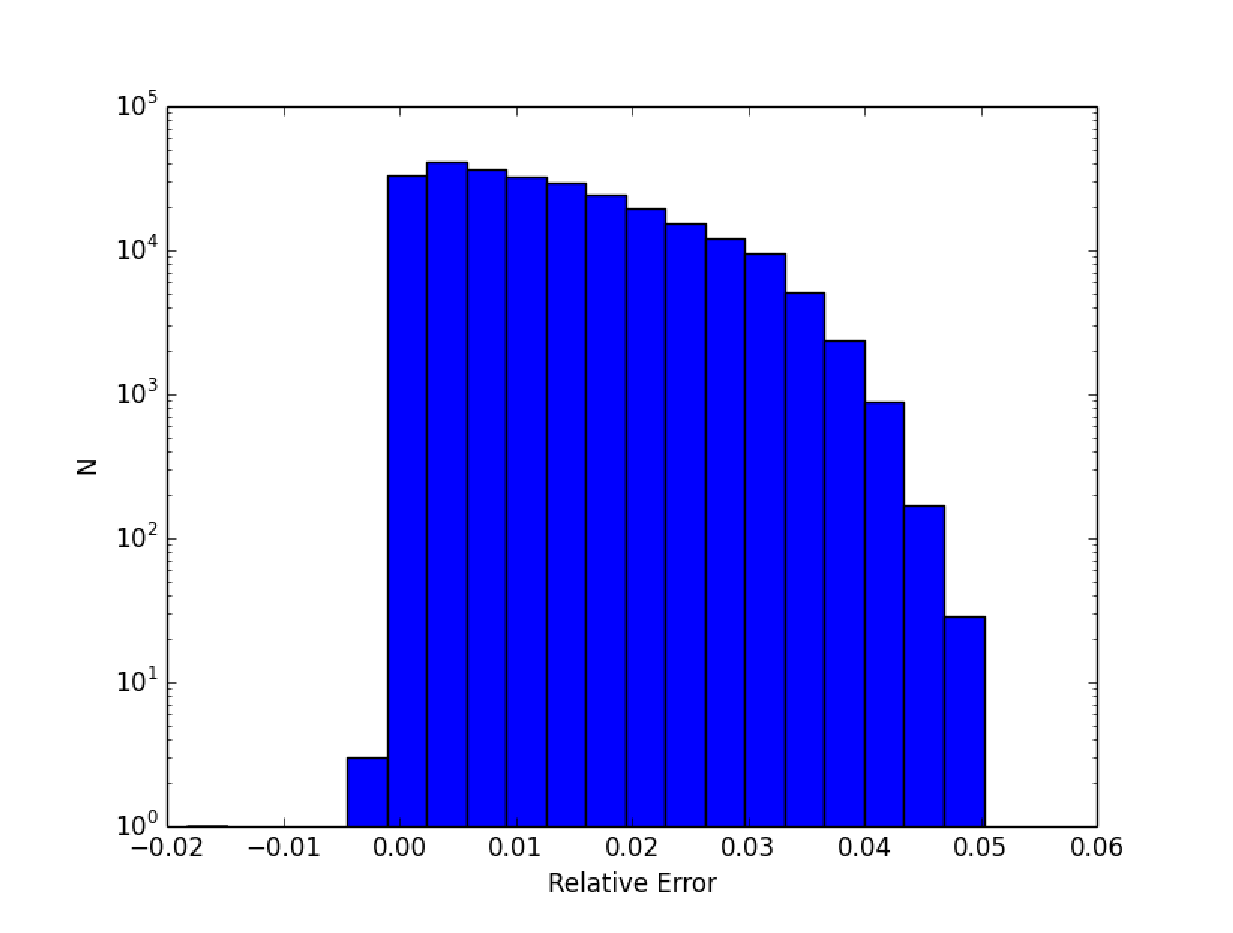
\includegraphics[width=\textwidth]{graphics/error.eps}
\caption[Error distribution for a single source in a uniform field.]{The distribution of flux errors among particles.}
\label{fig:thickglasserrors}
\end{figure}

\section{Multi-Source Glass}
\label{sec:multiglass}

We now show the effect of including many sources. The code is now performing at its most ``stressed;'' having a large number of randomly distributed sources means the code will run at its slowest and will include a large amount of averaging (not quite right).

\begin{itemize}
\item We first present the optically thin case. In this case, the glass has had half of its gas particles replaced with sources so that there are an equal number of each.
\item The error distribution present in this
\end{itemize}

\section{Effects of Averaging the Source}
\label{sec:averagingsource}

We now look closely at what effects averaging sources can have on results.

\subsection{Two star}
\label{sec:twostar}

\begin{figure}
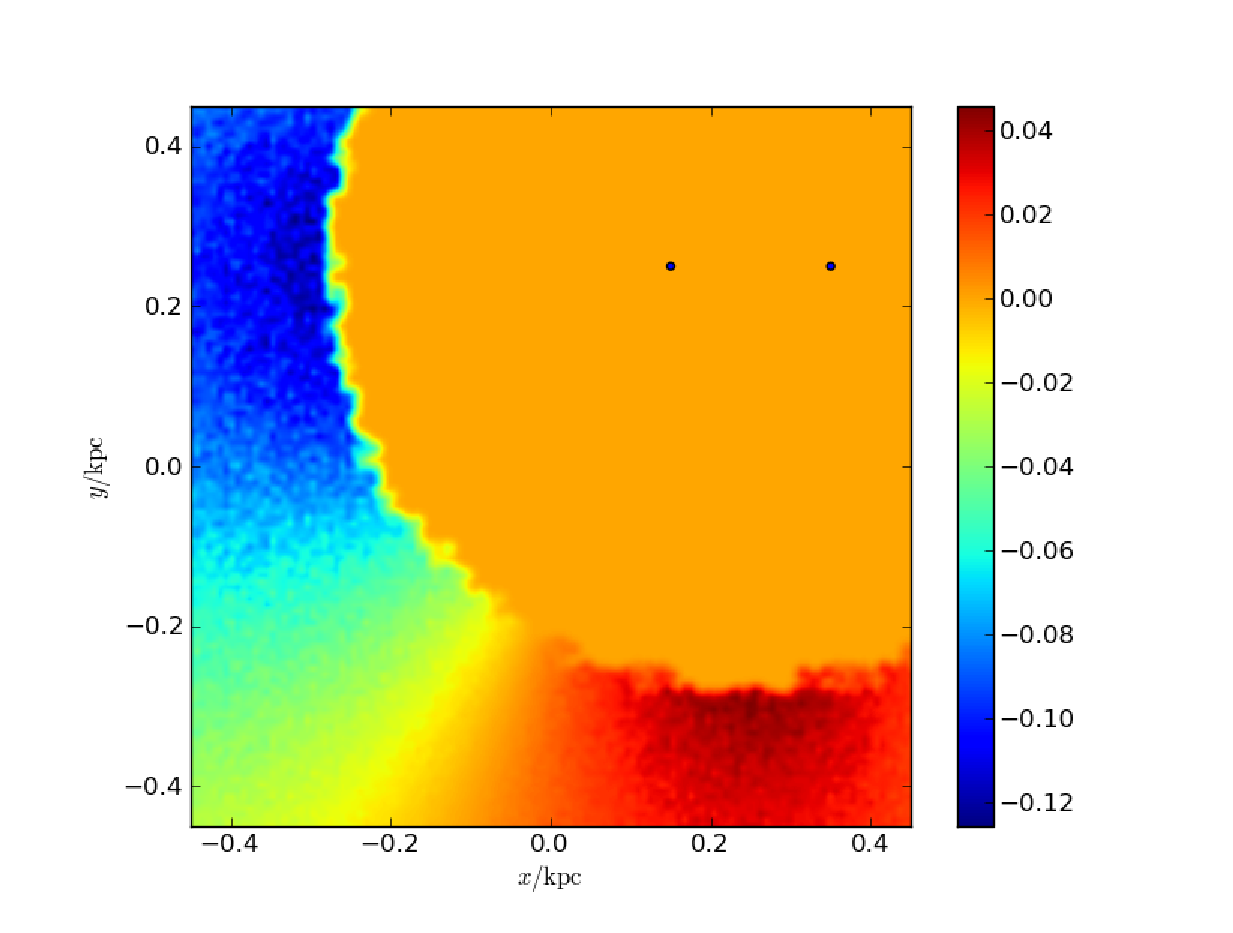
\includegraphics[width=\textwidth]{graphics/errorMap2starthick.eps}
\caption[The error associated with averaging star positions.]{The error associated with averaging star positions.}
\label{fig:twostar}
\end{figure}


\subsection{Isothermal Sphere with a Cluster(?)}
\label{sec:cluster}

Words

\section{The Str\"omgren Sphere}
\label{sec:stromgren}

The str\"omgren sphere is a theoretical ionized sphere of gas. It was first discussed by Bengt Str\"omgren in 1938 \citep{stromgren39}. We start with a cloud of homogeneous neutral Hydrogen gas and an ionizing source, commonly representing an O or B-type star, at the center. As the photons from the source ionize the hydrogen, the optical depth of the gas decreases, and so the ionizing photons move further out creating an ionization front. As the front moves out, the photon density as a function of radius falls off simply due to $1/r^2$ geometry and eventually a point is reached where the ionization rate falls to the recombination rate. At this point, the front stops in equilibrium.

One can solve for this radius by setting the photon density as a function of radius to the recombination rate and solving for radius \citep{stromgren39,spitzer78},

\begin{equation}
\label{eq:stromgrenradius}
R_S = \left( \frac{3}{4\pi} \frac{\dot{N_{\gamma}}}{\alpha n_H^2}\right).
\end{equation}

One can also find the growth rate of the front,

\begin{equation}
\label{eq:stromgrentime}
R(t) = R_S[1-\exp{(t/t_{\mbox{recomb}})}]^{1/3}.
\end{equation}

The above equations are the solutions for the evolution of a sharp ionization front, meaning that we have assumed the transition from ionized to neutral is infinitesimal in size. In order to solve for a non-sharp front, we must solve some equations numerically. FILL IN METHOD HERE.

\subsection{The Isothermal Case}
\label{sec:isostromgren}

In the simplest case, the ionizing source is assumed to emit photons at exactly 13.7 ev, meaning that the hydrogen gas is ionized but not heated. Cooling is also disabled, meaning that the gas is isothermal. If we assume that the ionization front propagates until the ionization rate drops low enough (due to geometric diminishment) to equal the recombination rate of the ambient medium, then we can solve for the equilibrium ionization radius by setting the two rates equal.

The ionization rate per unit volume can be written as the (fill in here)

%\begin{equation}
%\label{eq:fluxrecomb}
%F = \int_0^{r_s} n_e n_H \alpha_B(T) dl,
%\end{equation}
%
%where $n_e$ is the number density of electrons, $n_H$ is the number density of neutral Hydrogen, $\alpha_B$ is the case B recombination coefficient for Hydrogen for a given temperature, and $r_s$ is the equilibrium radius or ``Str\"omgren radius.'' 

\begin{equation}
\label{eq:strmogrenradius}
R_S = \left( \frac{3}{4\pi} \frac{\dot{N_{\gamma}}}{\alpha n_H^2}\right)
\end{equation}

\begin{equation}
\label{eq:stromgrentime}
R(t) = R_S[1-\exp{(t/t_{\mbox{recomb}})}]^{1/3}
\end{equation}

The above derivation assumes a ``sharp'' ionization front, meaning the transition from ionized to neutral is across an infinitesimal region. In practice, the transition region is small compared to the size of the ionized region, but there is structure interior to the Str\"omgren radius that is not accounted for by simply solving for the equilibrium radius. In order to solve for a non-sharp ionization front, we must integrate the above ionization equations \citep{osterbrockFerland2006}. (ADD HERE). In the following tests, we include both the sharp and non-sharp ionization front solutions for comparison to our results.

We follow the initial conditions of \citet{ilievEt2006}; the medium is initially neutral with a temperature 1e5 K and a density of 1e-3 cm$^{-3}$. An ionizing source is turned on at t = 0 that emits $\dot{N} = 5e48$ photons s$^{-1}$ at 13.6 ev. We use a cross section $\sigma = 6.3e-18 cm^2$ and a recombination rate of $\alpha = 2.59e-13 cm^{-3} s^{-1}$, typical of 1e5 K gas. These values give a Str\"omgren radius of 5.38 kpc and a recombination time of 125 Myr.

\begin{figure}
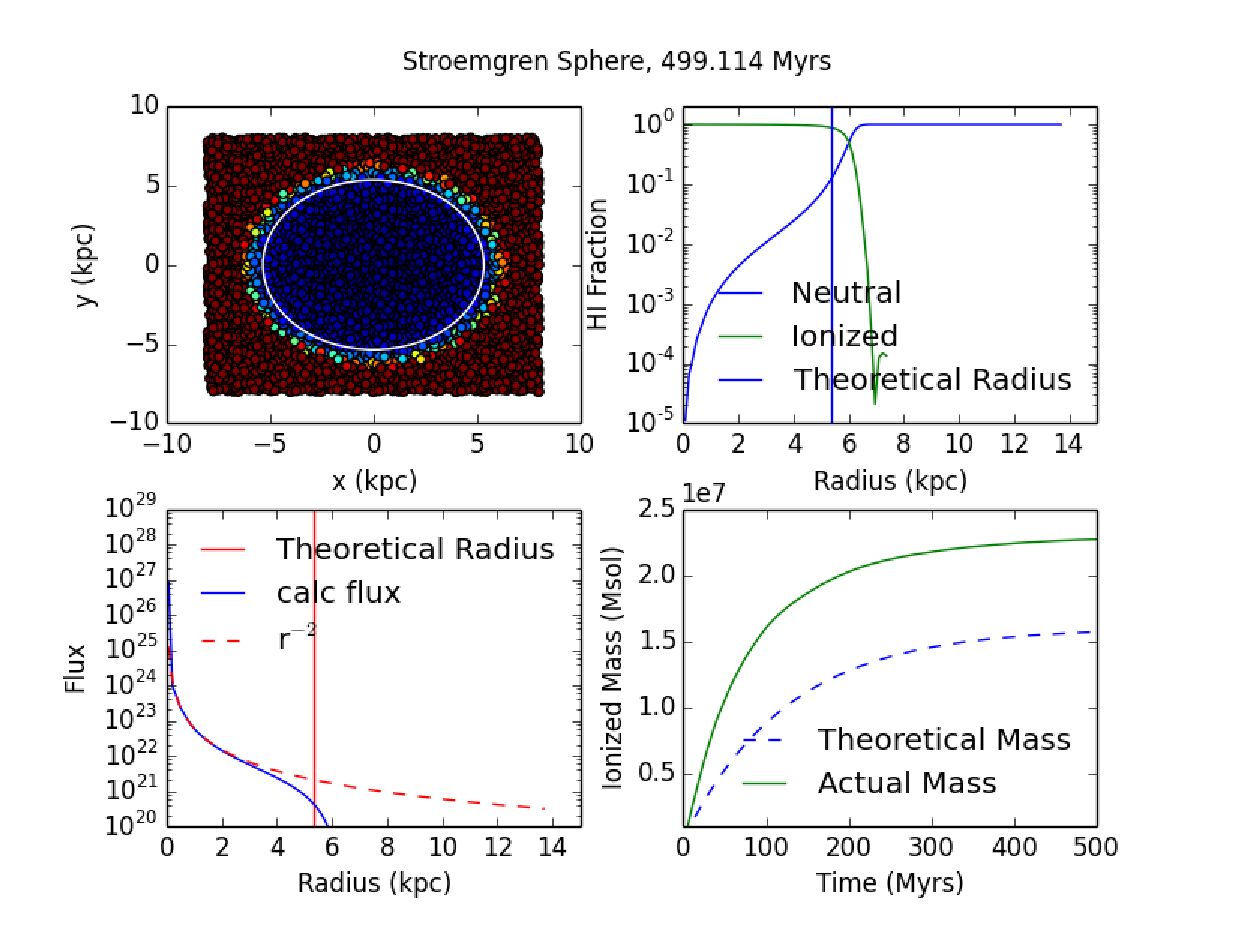
\includegraphics[width=\textwidth]{graphics/ifront6401000.eps}
\caption[The isothermal Str\"omgren Sphere.]{A slice of particles showing the ionization state.}
\label{fig:stromgreniso}
\end{figure}

\subsection{The Thermal Case}
\label{sec:thermalstromgren}

The above formulation assumed the gas was isothermal in order to simplify assumptions about cross section and recombination. In reality, both change with temperature. As well, the incoming photons are typically not all at a single wavelength but are distributed among many. The following test accounts for the latter factor, though not the former.

In this test, the incident photons are assumed to be from a black body with temperature 1e5 K. The cross section is changed to an integrated cross section, obtained by integrating the cross section as a function of wavelength over all wavelengths having energies between 13.6 ev and 29.65 ev.

\begin{figure}
        \centering
        \begin{subfigure}[b]{0.3\textwidth}
                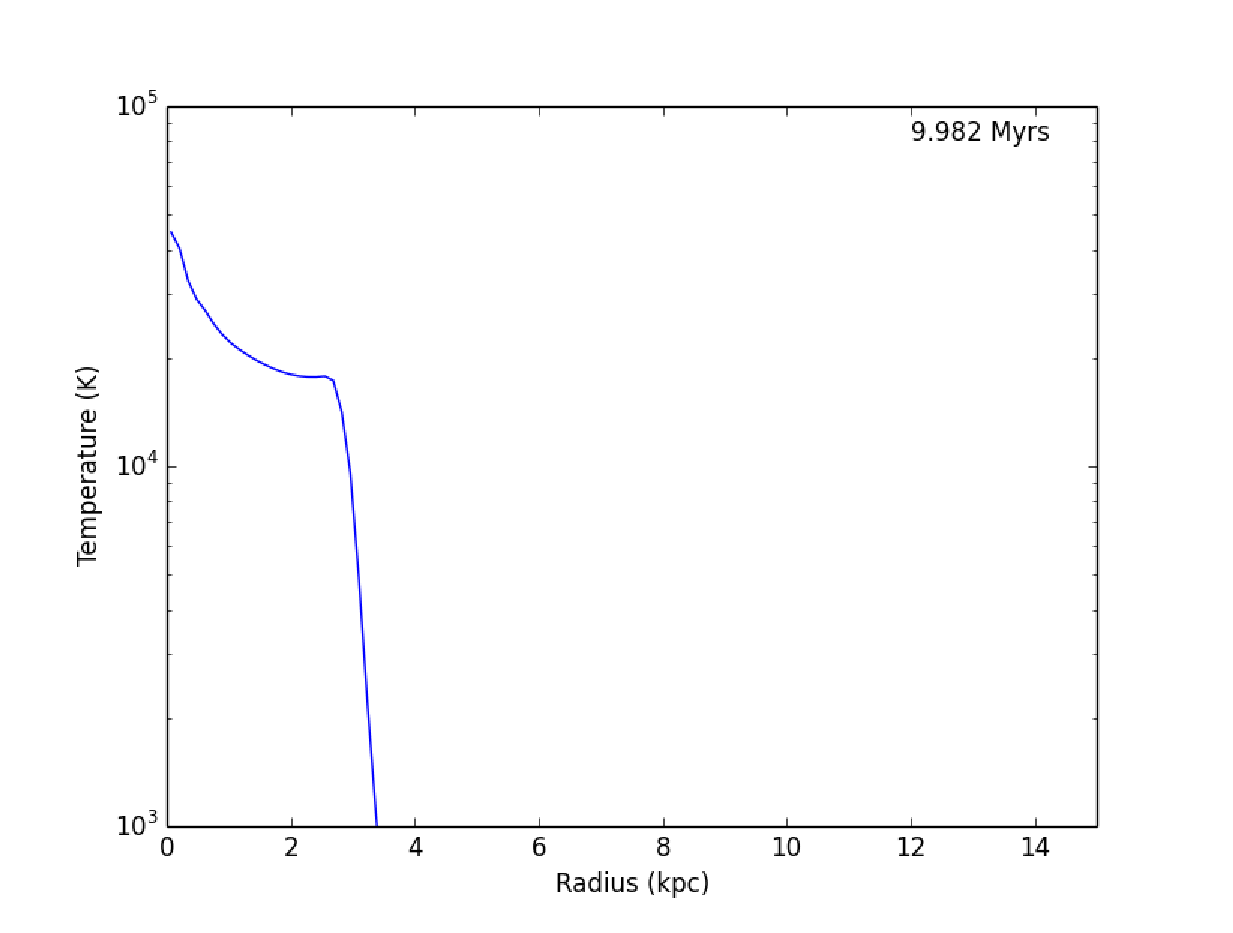
\includegraphics[width=\textwidth]{graphics/ifrontThermal6400020Tempprofile.eps}
                \label{fig:stromgrenthermal10}
        \end{subfigure}
        ~ 
        \begin{subfigure}[b]{0.3\textwidth}
                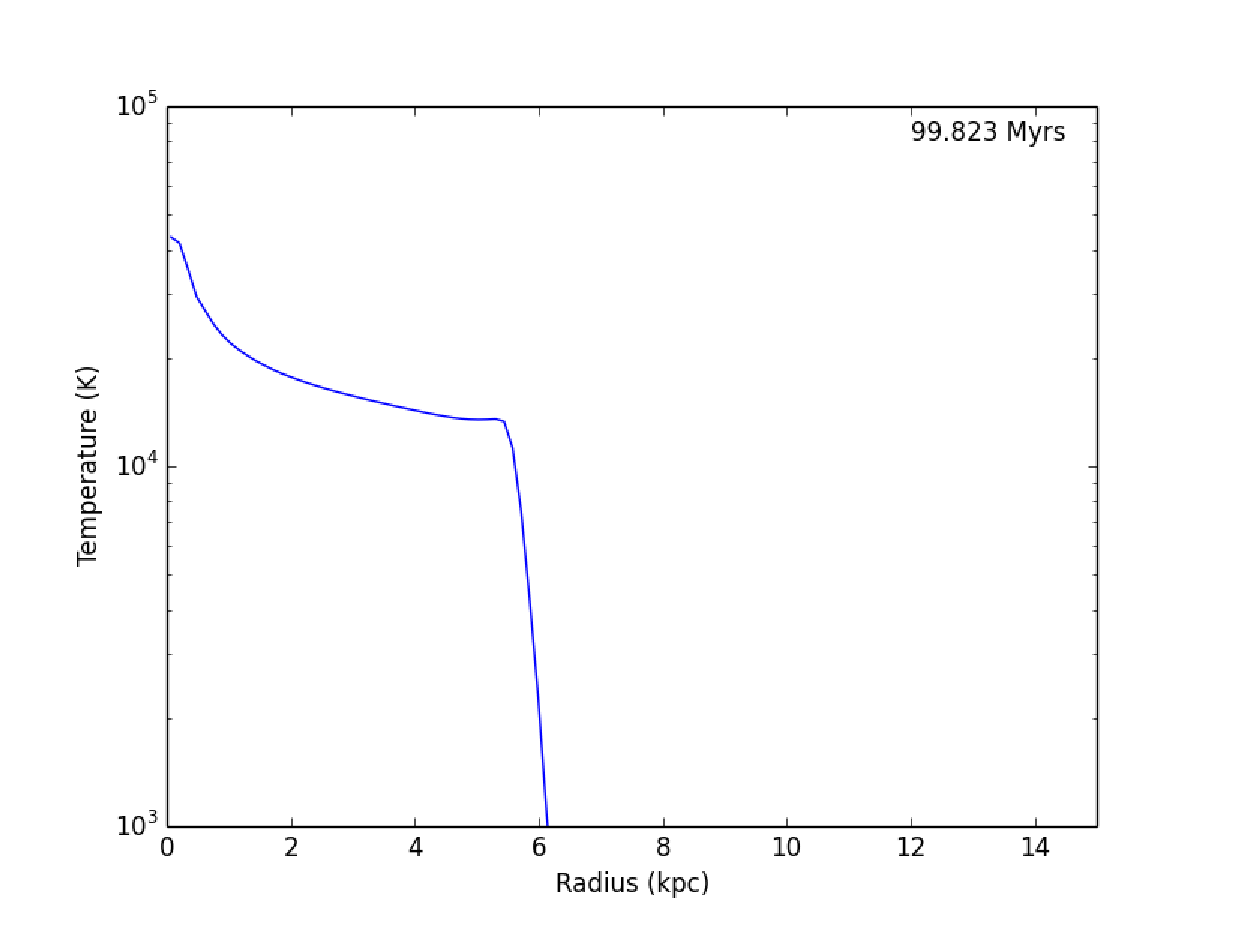
\includegraphics[width=\textwidth]{graphics/ifrontThermal6400200Tempprofile.eps}
                \label{fig:stromgrenthermal100}
        \end{subfigure}
        ~
        \begin{subfigure}[b]{0.3\textwidth}
                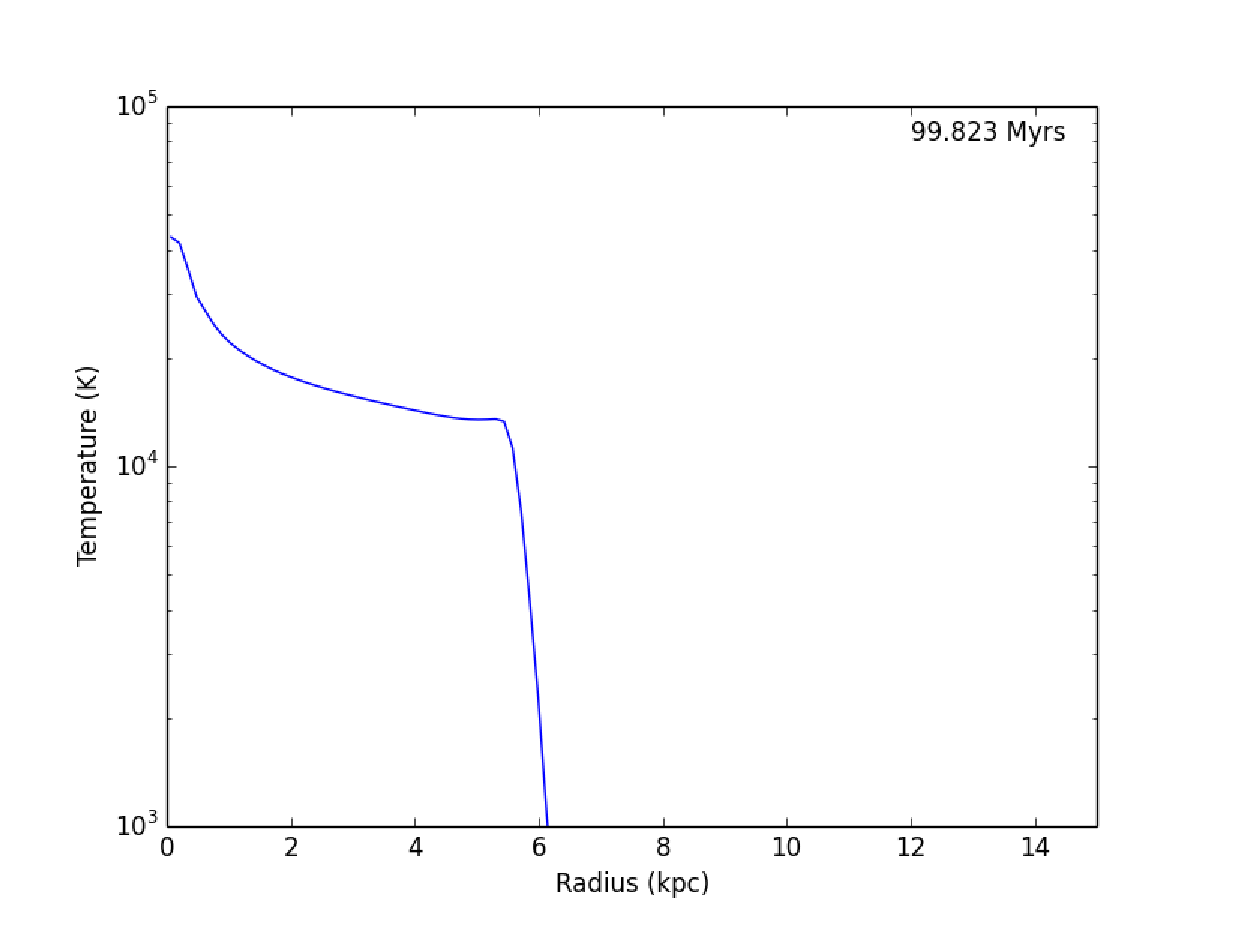
\includegraphics[width=\textwidth]{graphics/ifrontThermal6400200Tempprofile.eps}
                \label{fig:stromgrenthermal500}
        \end{subfigure}
        \caption[Temperature vs radius for the thermal Str\"omgren sphere.]{Temperature vs radius for the thermal Str\"omgren sphere.}
        \label{fig:stromgrenthermal}
\end{figure}

\section{The Gas Wall}
\label{sec:gaswall}

In order to test the algorithm's ability to handle a sharp density jump, we again perform the isothermal stromgren front (section \ref{sec:isostromgren}), but with a large density jump. We keep all of the same initial parameters, but change the density to the left of x = 0 to $\rho/2$ and the density to the right of x = 0 to $3/2 \rho$.

\subsection{Only Radiation}
\label{sec:gaswallradonly}

In the case that hydrodynamics is off, the solution is two stromgren hemispheres centered at x = 0.

\begin{figure}
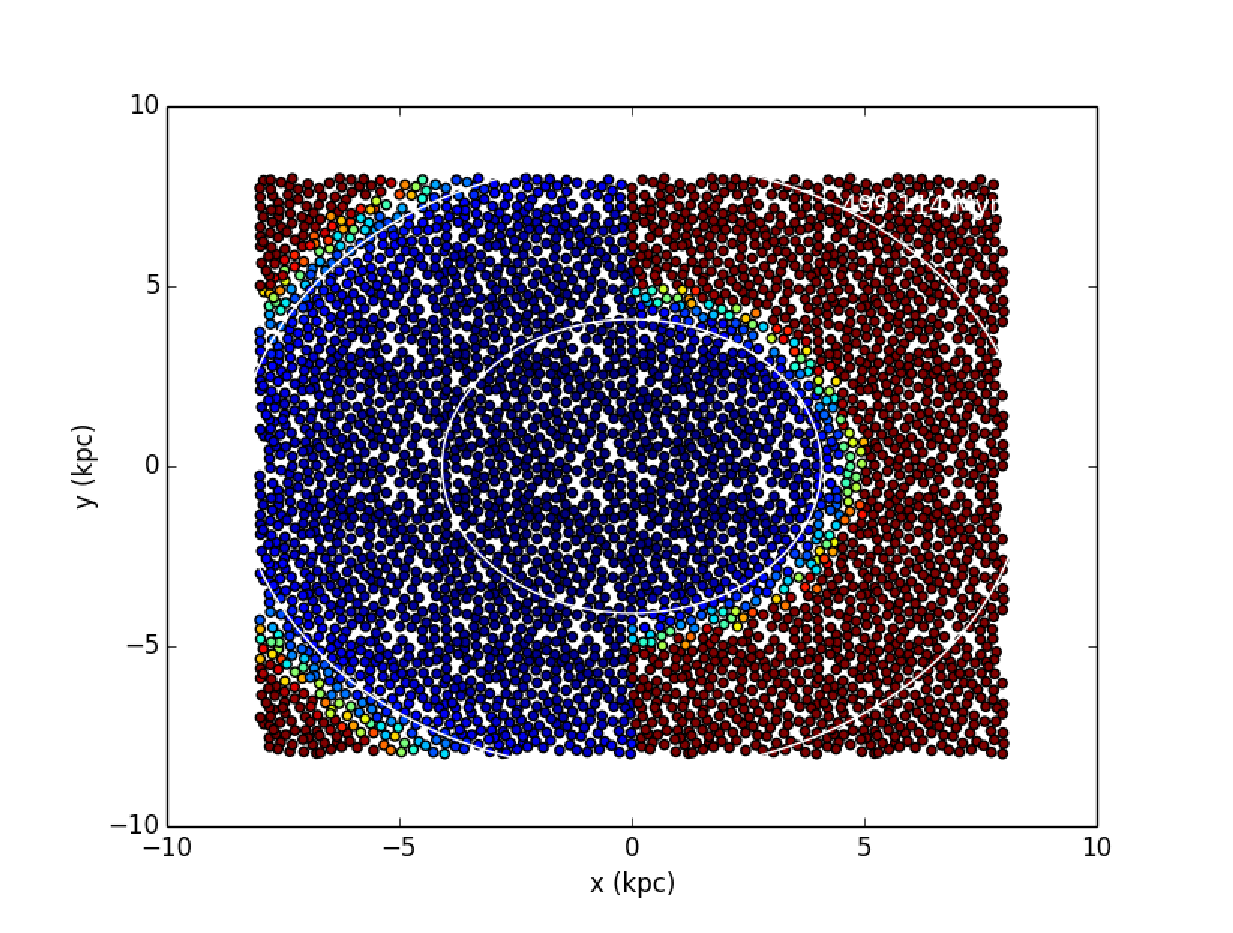
\includegraphics[width=\textwidth]{graphics/gasWall01000HIslice.eps}
\caption[Two slabs of gas at different densities.]{Two slabs of gas at different densities.}
\label{fig:gaswall}
\end{figure}


\subsection{With Hydrodynamics - the Champagne Flow}
\label{sec:champagne}

In order to test the coupling of radiation to the hydrodynamics, we perform a similar test in which the code now uses its hydrodynamics solvers. We follow the setup of \citet{gendelevKrumholz12}; A 50 pc cube is initialized with a density of 0.055 atoms cm$^{-3}$ to the right of x = 0, and 63 atoms cm$^{3}$ to the left. The temperatures of the left and right halves are 55 K and 6.3e3 K, respectively. This density/temperature combination gives pressure equilibrium at the boundary. An ionizing source is turned on at the origin that emits 5.3e47 photons/s, similar to a type BO.5 star. The combination of density and luminosity gives a stromgren sphere radius of 1.5 pc in the dense regions and a recombination time of 2.48e4 Years. The simulation is run for more than 4e6 years, meaning that the gas has time to heat and expand.

\begin{figure}
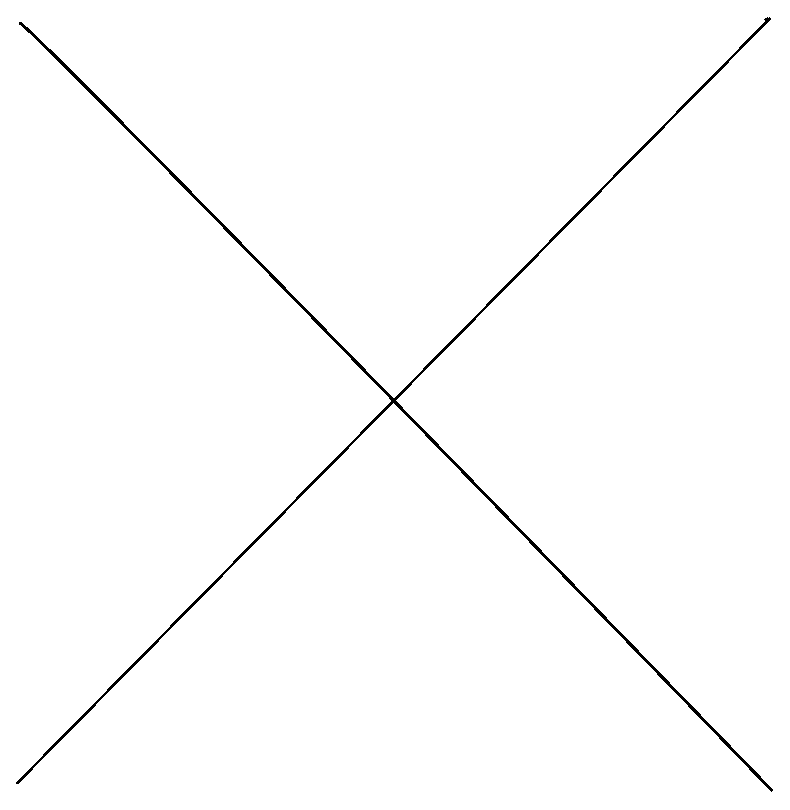
\includegraphics[width=\textwidth]{graphics/placeholder.eps}
\caption[An example of a champagne flow.]{An example of a champagne flow.}
\label{fig:champagne}
\end{figure}

\section{Shadowing}
\label{sec:shadowing}

Text to fix the formatting.

\begin{figure}
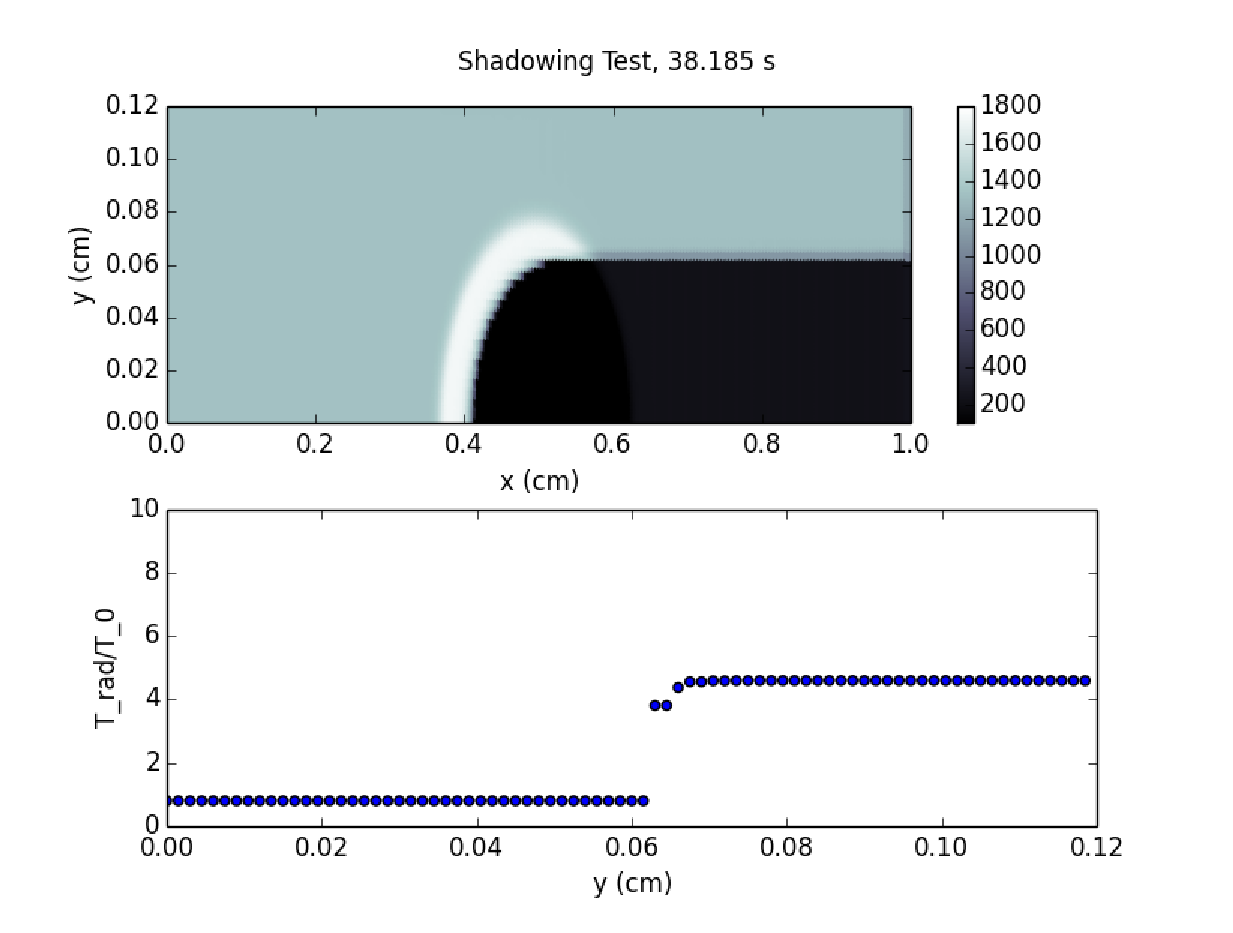
\includegraphics[width=\textwidth]{graphics/shadow10000.eps}
\caption[Shadowing.]{Demonstrating the codes ability to shadow.}
\label{fig:shadow}
\end{figure}

\section{Galaxy Disk}
\label{sec:galaxydisk}

Text to fix the formatting.

\section{Timings and Scaling}
\label{sec:timing}

Text to fix the formatting.

\begin{figure}
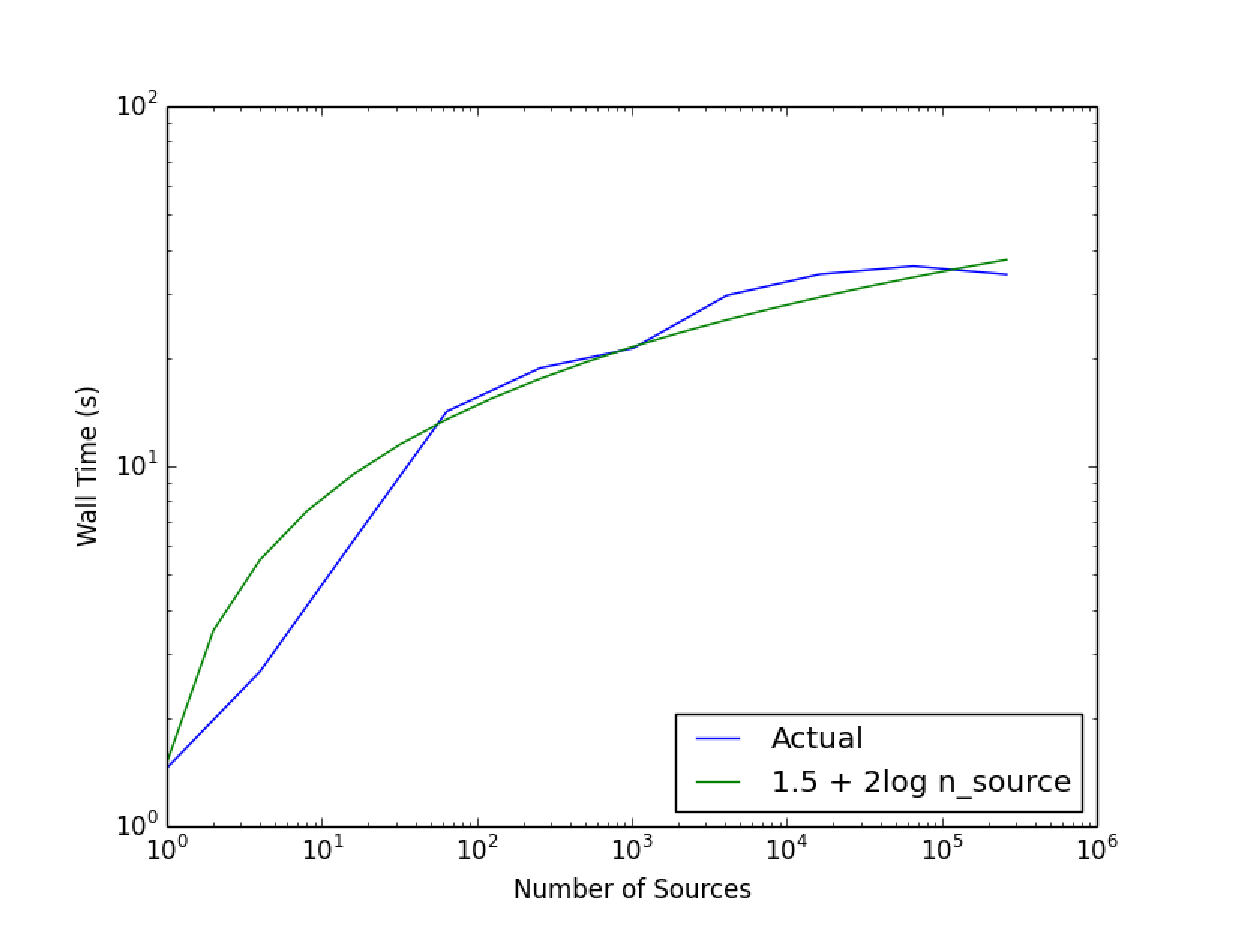
\includegraphics[width=\textwidth]{graphics/Timings.eps}
\caption[Wall time vs the number of sources.]{Wall time vs the number of sources.}
\label{fig:scaling}
\end{figure}


\pagestyle{fancy}
\headheight 20pt
\lhead{Ph.D. Thesis --- R. Woods }
\rhead{McMaster - Physics \& Astronomy}
\chead{}
\lfoot{}
\cfoot{\thepage}
\rfoot{}
\renewcommand{\headrulewidth}{0.1pt}
\renewcommand{\footrulewidth}{0.1pt}

\chapter{Applications to Galaxy Formation and Future Projects}
\label{chap:galaxyformation}
\thispagestyle{fancy}

We now use the algorithm described in chapter \ref{chap:method} and tested in chapter \ref{chap:codetests} to carry out simulations of an isolated galaxy. We have chosen to start with an isolated galaxy in order to probe the FUV field present in a [Milky Way-like... z=1?] disk in order to check if it is an important SF regulation mechanism.

FUV is an interesting band to start with for a few reasons. While FUV does not ionize gas, it is the primary driver of photoelectric heating \citep{tielens05}, which is the dominant heating mechanism for the ISM and the warm neutral medium. Despite this, very few astrophysical simulations actually include photoelectric heating due to its dependence on a radiation field.

As well, FUV is typically able to penetrate further into the ISM. At common densities in the ISM, an optical depth of 1 is typically only achieved after roughly one kpc. Current simulations, especially of isolated galaxies, can resolve distances much smaller than this, so looking at effects due to FUV is very feasible. On the other hand, bands such as EUV are usually absorbed within a few pc, a resolution that is very costly for even isolated galaxy simulations.

We have chosen to use an isolated galaxy IC from the AGORA galaxy comparison project \citep{kimEt14} to ensure use of a well-tested IC and provide a larger base for comparison of results.

\section{FUV Fields in the AGORA Disk}
\label{sec:agora}

The AGORA galaxy comparison project is a large computational comparison project that aims ``to raise the realism and predictive power of galaxy simulations and the understanding of the feedback processes that regulate galaxy `metabolism,' and by doing so to solve long-standing problems in galaxy formation'' \citep{kimEt14}. To accomplish this, the project has created both isolated and cosmological galaxy formation initial conditions at many different masses and resolutions, and has attempted to standardize physics modules and analysis methods for all of the codes involved in the project.

\subsection{Initial Conditions and Physics}
\label{sec:initialconditions}

We have chosen to run the isolated disk initial condition in order to examine FUV's effect on the ISM. The specific details of the ICs for this disk can be found in \citet{kimEt14}, section 2.2. We summarize here the important information.

The initial conditions have been generated at three different resolutions using the \textsc{MakeDisk} code, written by Volker Springel. The disk is created with four components: a dark matter halo, a gas disk, a stellar disk, and stellar bulge. The low resolution disk has $10^5$ DM particles, $10^5$ stellar disk particles, $10^5$ gas particles, and $1.24\e{4}$ stellar bulge particles. The medium and high resolution disks have 10 and 100 times more particles in each component, respectively.

The DM follows a NFW profile \citep{navarroEt97} with a concentration parameter $c = 10$ and a spin parameter $\lambda = 0.04$. The disk has an exponential profile with a scale length of $r_d = 3.432$ kpc and a scale height of $z_d = 0.1 r_d$. The disk is split into the stellar component, which has a mass of $4.297\e{10} M_{\odot}$, and a gas component, which has a mass of 20\% of the DM mass. The stellar bulge follows the Hernquist \citeyear{hernquist90} density profile with a bulge-to-disk mass ratio of B/D = 0.1. Gas is initiated at $10^4$ K. The \textsc{MakeDisk} code ensures that the above conditions give quasi-equilibrium [what does that mean?] for the four components. An image of the IC is shown in figure \ref{fig:agoraic}.

\begin{figure}
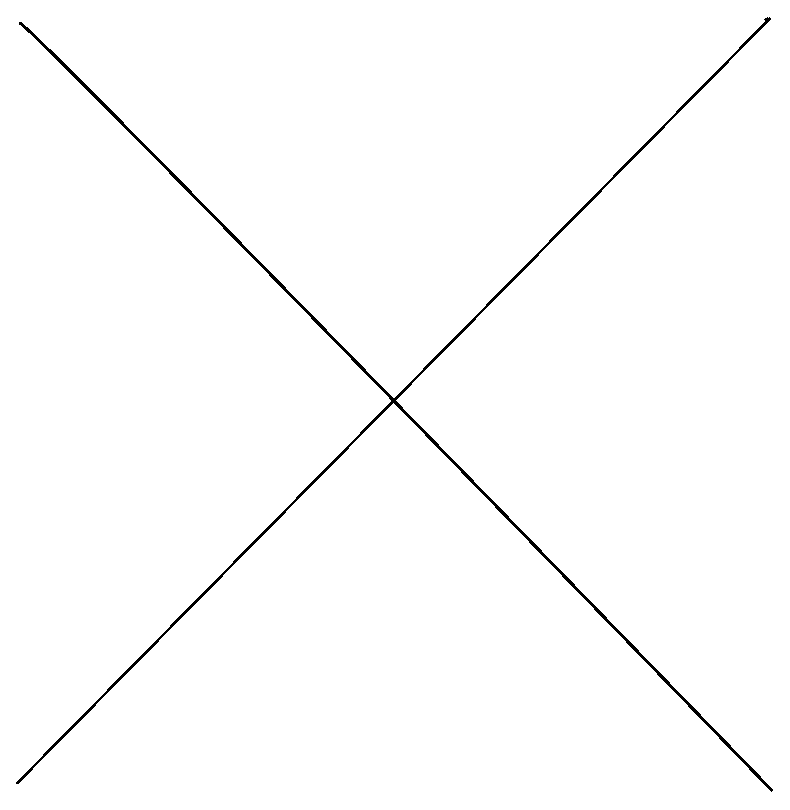
\includegraphics[width=\textwidth]{graphics/placeholder.eps}
\caption[The AGORA IC]{A density slice in the z plane of the AGORA initial condition.}
\label{fig:agoraic}
\end{figure}

%notes about various runs we did

We have run the low resolution simulation with a number of different physical parameters, including our radiative transfer with FUV, a background FUV at two intensities (the standard for most codes without radiative transfer), and Supernovae (SNe) feedback \citep{kellerEt14}. Table \ref{tab:simsummary} summarizes the simulations and the names we have given them.

\begin{table}
\begin{tabular}{llll}
Name & RT & UV Strength (units?) & SNe Feedback\\ \hline \hline
RadFUV & Yes & 0 & No\\
RadFUV2e-26 & No & 2e-26 & No\\
RadFUV2e-27 & No & 2e-27 & No\\
RadFB & No & ? & yes\\
RadFB\_FUV & Yes & 0 & yes\\
RadFB\_FUV2e-26 & No & 2e-26 & yes\\
RadFB\_FUV2-27 & No & 2e-27 & yes\\
\hline
\end{tabular}
\caption[Summary of simulations]{A summary of the simulations that were run.}
\end{table}

We have also included a run at medium resolution to check on convergence of results. It is important to note that resolution may play an important factor in the following results. \citet{FILL IN} [ask sam for references] found that in order to get proper ISM behavior, a simulation needs to be at a high enough resolution. As will be noted in section \ref{sec:futurework}, a convergence study in resolution should be performed on this work.

\section{The Role of FUV on Star Formation}
\label{sec:fuvsfr}


We begin by looking at the star formation history of each simulation. Figure \ref{fig:sfrvtime} shows the star formation rate as a function of time for each simulation. 

\begin{figure}
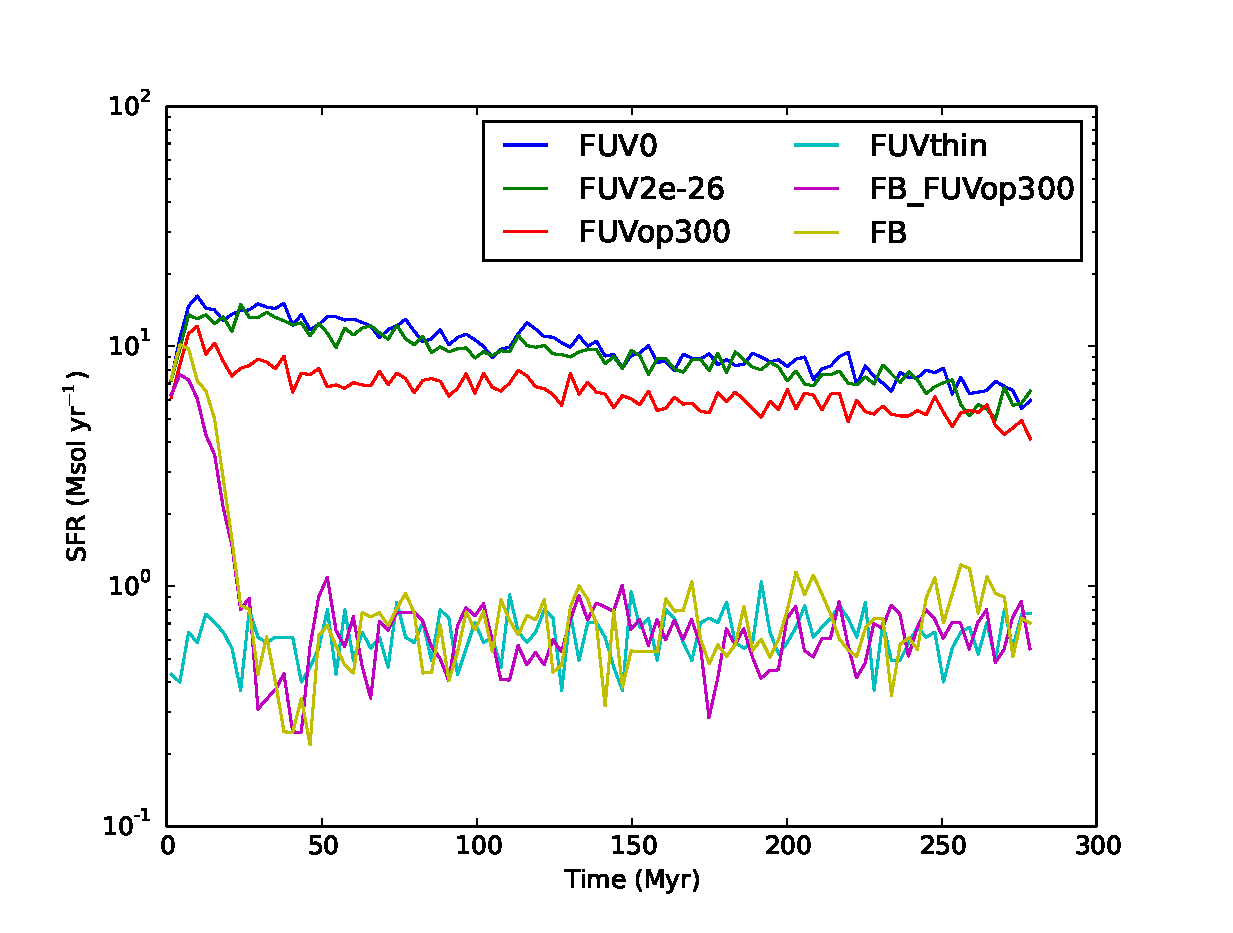
\includegraphics[width=\textwidth]{graphics/sfrvtime.eps}
\caption[Star formation histories.]{Star formation rate vs time for each simulation. Feedback dominates the star formation regulation in this galaxy. Looking only at FUV, local feedback has a noticeable effect over a uniform background UV field.}
\label{fig:sfrvtime}
\end{figure}

It is clear that SNe feedback has a very strong regulation effect on star formation, as the rate in all runs with SNe feedback is about a factor of five lower than simulations without SNe feedback. In runs without SNe feedback, local FUV fields tend to reduce star formation rates by a factor of around 25\% compared to uniform backgrounds. Comparing the RadFUV2e-26 and RadFUV2e-27, there is no noticeable difference, suggesting that the FUV due to a uniform background has no ability to regulate star formation.

We must check whether the FUV field present in the galaxy is similar to observations. Figure \ref{fig:intensitywolfire} is a plot of FUV intensity vs radius in the midplane of the galaxy.

\begin{figure}
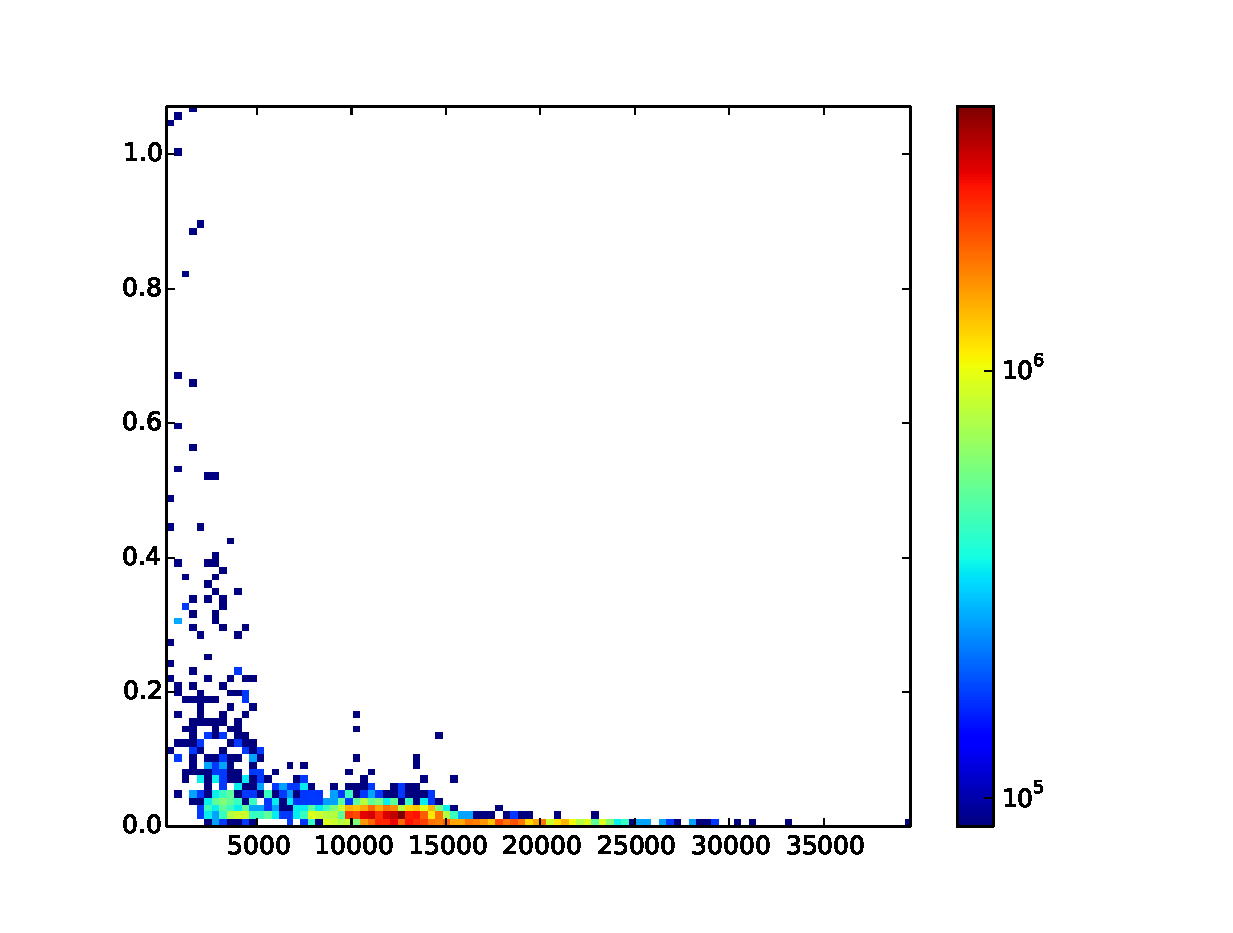
\includegraphics[width=\textwidth]{graphics/intensityvrRadFB_FUV00101.eps}
\caption[FUV intensity vs radius]{FUV intensity vs radius in the galaxy midplane for the RadFUV case. The dots are individual particle fluxes and the solid line is from figure 5.5 of \citet{wolfireEt03}.}
\label{fig:intensitywolfire}
\end{figure}

The points are intensities for individual particles and the lines is the mean intensity presented in \citet{wolfireEt03}. On average, the FUV intensity seen by a particle is far lower than the mean field presented by \citet{wolfireEt03}.

In order to understand the affect FUV has on gas, we consider phase diagrams for gas in the galaxy. Figure \ref{fig:phasediagrams} shows phase diagrams of gas in a number of the different simulations.

\begin{figure}
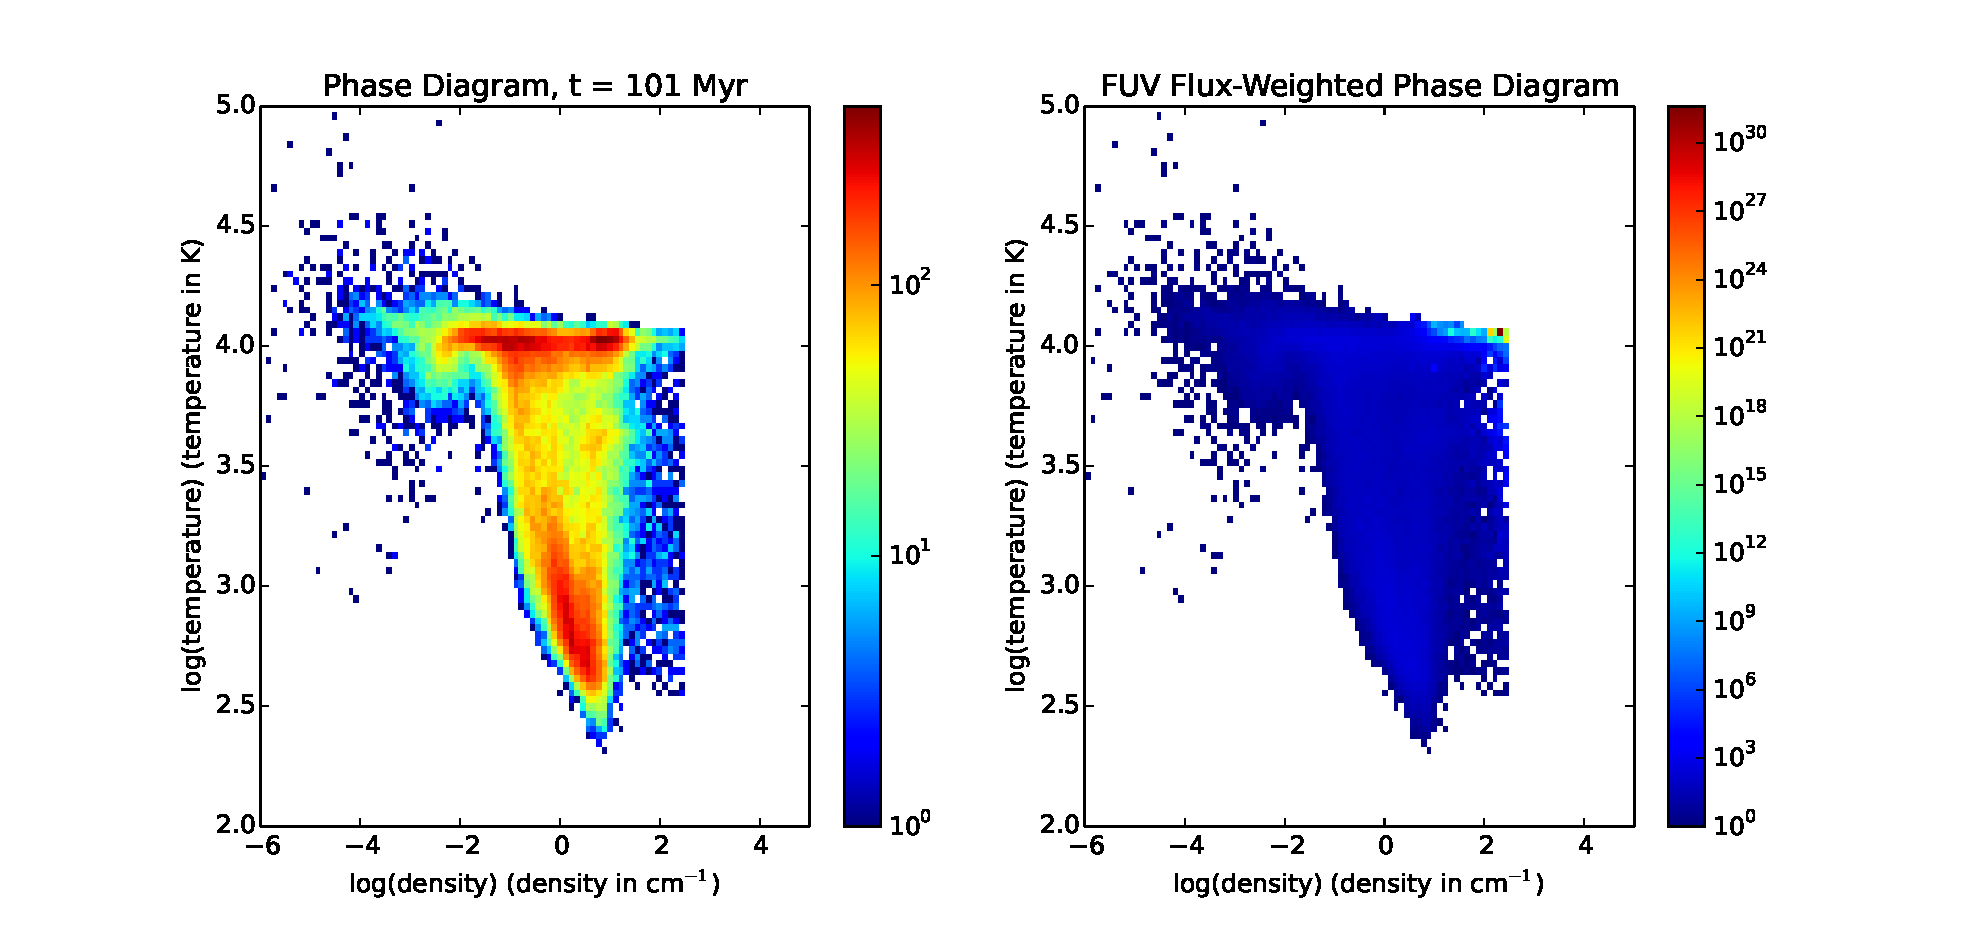
\includegraphics[width=\textwidth]{graphics/phaseRadFUV00101.eps}
\caption[Phase diagrams with different physics]{Phase diagrams for each simulation case.}
\label{fig:phasediagrams}
\end{figure}

In cases with FUV simulated with radiative transfer, a portion of the gas is seen to be heated to about $10^4$ K around densities of 100 atoms cm$^{-3}$.

\section{Future Projects [Move to Ch 6?]}
\label{sec:futurework}

\subsection{Astrophysics Projects}
\label{sec:astroprojects}

Future work of this algorithm is quite broad; the flexibility allows application to a wide range of problems. An immediate follow up is to the work presented in section \ref{sec:agora}. [Author] suggests that four radiation bands, HI ionization, He ionization, LyWerner, and CI, are needed to sufficiently recreate ISM properties. Using these four bands, we would like to calculate the effect of radiation on the ISM. Including these four sources of heating and ionization will enable classification of which bands regulate star formation as a function of environment, and which bands drive particular phases of the ISM.

Currently, there is very little work in computational astrophysics that models the UV fields in and around galaxies. While many models have been created from the observational side [references], due to large computational cost, simulations have left this area largely unexplored or explored only at high redshift [references].

The next project for the radiative transfer code will be to include UV in the McMaster Unbiased Galaxy Simulations 2 (MUGS2) simulations. The MUGS2 project is a set of cosmological simulations of galaxies spanning a large range of parameter space. There are currently [16] galaxies in the set spanning a mass range of $5\e{11} M_{\odot}$ to $2\e{12} M_{\odot}$. Including explicit radiative transfer in these cosmological simulations all the way down to redshift zero would be an unprecedented accomplishment in computational galaxy formation. The group of simulations would enable comparison of the effectiveness of radiative transfer in transforming and regulating galaxy formation across a wide mass range at different epochs in time.

Having a wide range of simulated galaxies all with RT will also enable a plethora of other analysis. Currently, escape fractions of radiation from galaxies are typically assumed to be certain values (e.g. \citet{kannanEt14}). With the MUGS2 simulations including RT, escape fractions could be explicitly calculated.

\textsc{Gasoline} has a chemical network for molecular Hydrogen (H2) creation and destruction \citep{christensenEt12}, but requires an accurate Lyman-Werner field in order to be used. The new RT can provide this, and enables studies on H2 formation and destruction in galaxies, as well as studies of H2 shielding, self and dust, in molecular clouds. This has the additional advantage of easily being linked to observations.

We note that a potential application is to study cosmic re-ionization. However, this application may not be as ideal. Besides having already received a fair bit of attention from simulators, our code does not explicitly conserve photons and so does not guarantee correct ionization front propagation speeds, which are quite important for studies of cosmic re-ionization.

Finally, an exciting potential application is to look at re-radiation of photons from gas. This could include the effects of gas re-radiating ionizing photons when electrons recombine back to the ground state. This effectively increases the penetration depth of ionizing photons and can have an important effect on the gas in the ISM at particular densities [cite rahmati]. As well, processing of stellar emission down to IR wavelengths could be a very interesting study. However, both of these applications rely on a successful implementation of gas radiation in \textsc{Gasoline}. While in principle the implemented RT can handle any radiation, allowing gas to radiate requires care in that it must be self-consistently tied to the cooling that gas experiences. At first glance, separating cooling and cooling radiation induces a cooling instability and so requires further investigation to be done properly (see section \ref{sec:codeadditions}).

\subsection{Code Additions}
\label{sec:codeadditions}

The algorithm we have presented is very flexible, efficient, and powerful. However, there is a lot of room for improvement in the algorithm and optimizations that can be made.

For example, if it is know a priori that all sources lie outside of the absorbing material, the algorithm can be simplified to run in order $N\log{N}$ time by implementing the algorithm presented in TreeCOL \citep{clarkEt12}. In this scenario, each receiving leaf partitions the rest of the tree into equal areas on the sky (TreeCOL uses the HEALPIX algorithm \citep{gorskiEt05}, but it is not required) during the tree walk. Since an effective size of each cell the leaf interacts with can be calculated, each cell can add its absorption contributions to the proper area on the leaf's sky map.

It is also possible to make optimizations in the tree build process. Currently, the tree is rebuilt for every substep the simulation takes, regardless of how large the time step is. It's possible to simply ``fix'' the tree rather than rebuilding it in cases where particles have not moved by much [cite codes that do this]. Along the same lines, it's also possible to avoid recalculating radiation if the time step is very small. If particles have not moved by much and radiation sources have not been significantly changed, than there is no reason to recalculate the radiation field. This would require flagging of ``unimportant'' regions or including a radiation-set time step in the code. If the code time step was smaller than the radiation time step, then the radiation calculation could be skipped.

Currently, the algorithm supports an arbitrary number of wave bands. However, work is still needed to couple the photons in these bands to cooling and heating processes in the code. Adding this functionality will greatly open up the number of projects the algorithm can be used for.

It would also be very interesting to create the ability to use gas particles as sources. This enables the code to treat re-radiation by gas, dust emission, and potentially even scattering if a gas particle's emission in one band was based on its incident intensity in another band. Due to the excellent scaling with the number of sources that the algorithm provides, this should not be computationally prohibitive. The consideration to make here is how self consistent the cooling is with radiation. For example, if a gas particle emits a certain luminosity in certain bands, but the cooling code integrates out a different cooling rate, energy conservation can be violated, and cooling instabilities in the gas particle can be created [more details here]. This code addition will require special attention to get right.

Other minor features can be added without too much difficulty. For example, radiation is currently not allowed to be periodic. However, there is no reason a tree cell cannot be copied in a similar way to gravitational periodicity (where an offset is simply added to each cell in the tree to represent a periodic copy). As well, it is possible to add dynamical effects due to radiation such as radiation pressure. This simply requires code to be added into the acceleration calculations to use the radiation field information.

[closing statement?]
\pagestyle{fancy}
\headheight 20pt
\lhead{Ph.D. Thesis --- R. Woods }
\rhead{McMaster - Physics \& Astronomy}
\chead{}
\lfoot{}
\cfoot{\thepage}
\rfoot{}
\renewcommand{\headrulewidth}{0.1pt}
\renewcommand{\footrulewidth}{0.1pt}

\chapter{Conclusions and Future Work}
\label{chap:conclusions}
\thispagestyle{fancy}


\section{Future Projects}
\label{sec:futurework}

\subsection{Astrophysics Projects}
\label{sec:astroprojects}

Future work of this algorithm is quite broad; the flexibility allows application to a wide range of problems. An immediate follow up is to the work presented in section \ref{sec:agora}. [Author] suggests that four radiation bands, HI ionization, He ionization, LyWerner, and CI, are needed to sufficiently recreate ISM properties. Using these four bands, we would like to calculate the effect of radiation on the ISM. Including these four sources of heating and ionization will enable classification of which bands regulate star formation as a function of environment, and which bands drive particular phases of the ISM.

Currently, there is very little work in computational astrophysics that models the UV fields in and around galaxies. While many models have been created from the observational side [references], due to large computational cost, simulations have left this area largely unexplored or explored only at high redshift [references].

The next project for the radiative transfer code will be to include UV in the McMaster Unbiased Galaxy Simulations 2 (MUGS2) simulations. The MUGS2 project is a set of cosmological simulations of galaxies spanning a large range of parameter space. There are currently [16] galaxies in the set spanning a mass range of $5\e{11} M_{\odot}$ to $2\e{12} M_{\odot}$. Including explicit radiative transfer in these cosmological simulations all the way down to redshift zero would be an unprecedented accomplishment in computational galaxy formation. The group of simulations would enable comparison of the effectiveness of radiative transfer in transforming and regulating galaxy formation across a wide mass range at different epochs in time.

Having a wide range of simulated galaxies all with RT will also enable a plethora of other analysis. Currently, escape fractions of radiation from galaxies are typically assumed to be certain values (e.g. \citet{kannanEt14}). With the MUGS2 simulations including RT, escape fractions could be explicitly calculated.

\textsc{Gasoline} has a chemical network for molecular Hydrogen (H2) creation and destruction \citep{christensenEt12}, but requires an accurate Lyman-Werner field in order to be used. The new RT can provide this, and enables studies on H2 formation and destruction in galaxies, as well as studies of H2 shielding, self and dust, in molecular clouds. This has the additional advantage of easily being linked to observations.

We note that a potential application is to study cosmic re-ionization. However, this application may not be as ideal. Besides having already received a fair bit of attention from simulators, our code does not explicitly conserve photons and so does not guarantee correct ionization front propagation speeds, which are quite important for studies of cosmic re-ionization.

Finally, an exciting potential application is to look at re-radiation of photons from gas. This could include the effects of gas re-radiating ionizing photons when electrons recombine back to the ground state. This effectively increases the penetration depth of ionizing photons and can have an important effect on the gas in the ISM at particular densities [cite rahmati]. As well, processing of stellar emission down to IR wavelengths could be a very interesting study. However, both of these applications rely on a successful implementation of gas radiation in \textsc{Gasoline}. While in principle the implemented RT can handle any radiation, allowing gas to radiate requires care in that it must be self-consistently tied to the cooling that gas experiences. At first glance, separating cooling and cooling radiation induces a cooling instability and so requires further investigation to be done properly (see section \ref{sec:codeadditions}).

\subsection{Code Additions}
\label{sec:codeadditions}

The algorithm we have presented is very flexible, efficient, and powerful. However, there is a lot of room for improvement in the algorithm and optimizations that can be made.

For example, if it is know a priori that all sources lie outside of the absorbing material, the algorithm can be simplified to run in order $N\log{N}$ time by implementing the algorithm presented in TreeCOL \citep{clarkEt12}. In this scenario, each receiving leaf partitions the rest of the tree into equal areas on the sky (TreeCOL uses the HEALPIX algorithm \citep{gorskiEt05}, but it is not required) during the tree walk. Since an effective size of each cell the leaf interacts with can be calculated, each cell can add its absorption contributions to the proper area on the leaf's sky map.

It is also possible to make optimizations in the tree build process. Currently, the tree is rebuilt for every substep the simulation takes, regardless of how large the time step is. It's possible to simply ``fix'' the tree rather than rebuilding it in cases where particles have not moved by much [cite codes that do this]. Along the same lines, it's also possible to avoid recalculating radiation if the time step is very small. If particles have not moved by much and radiation sources have not been significantly changed, than there is no reason to recalculate the radiation field. This would require flagging of ``unimportant'' regions or including a radiation-set time step in the code. If the code time step was smaller than the radiation time step, then the radiation calculation could be skipped.

Currently, the algorithm supports an arbitrary number of wave bands. However, work is still needed to couple the photons in these bands to cooling and heating processes in the code. Adding this functionality will greatly open up the number of projects the algorithm can be used for.

It would also be very interesting to create the ability to use gas particles as sources. This enables the code to treat re-radiation by gas, dust emission, and potentially even scattering if a gas particle's emission in one band was based on its incident intensity in another band. Due to the excellent scaling with the number of sources that the algorithm provides, this should not be computationally prohibitive. The consideration to make here is how self consistent the cooling is with radiation. For example, if a gas particle emits a certain luminosity in certain bands, but the cooling code integrates out a different cooling rate, energy conservation can be violated, and cooling instabilities in the gas particle can be created [more details here]. This code addition will require special attention to get right.

Other minor features can be added without too much difficulty. For example, radiation is currently not allowed to be periodic. However, there is no reason a tree cell cannot be copied in a similar way to gravitational periodicity (where an offset is simply added to each cell in the tree to represent a periodic copy). As well, it is possible to add dynamical effects due to radiation such as radiation pressure. This simply requires code to be added into the acceleration calculations to use the radiation field information.

[closing statement?]

\section{Conclusions}
\label{sec:conclusion}

Deep thoughts here.

%\end{singlespace}
\end{doublespace}


%%%%%%%%%%%%%%%%%%%%%%%%%%%%%%%%%%%%%%%%%%%%%%%%%%%%%%%%%%%%%%%
%Appendices
%%%%%%%%%%%%%%%%%%%%%%%%%%%%%%%%%%%%%%%%%%%%%%%%%%%%%%%%%%%%%%%
\appendix
\pagestyle{fancy}
\headheight 20pt
\lhead{PhD Thesis --- M. Klassen }
\rhead{McMaster Physics and Astronomy}
\chead{}
\lfoot{}
\cfoot{\thepage}
\rfoot{}
\renewcommand{\headrulewidth}{0.1pt}
\renewcommand{\footrulewidth}{0.1pt}

\chapter{Appendix A} \label{Appendix-A} 
\thispagestyle{fancy} 






%%%%%%%%%%%%%%%%%%%%%%%%%%%%%%%%%%%%%%%%%%%%%%%%%%%%%%%%%%%%%%%
% ESM students need to include a Nontechnical Abstract as the %
% last appendix.                                              %
%%%%%%%%%%%%%%%%%%%%%%%%%%%%%%%%%%%%%%%%%%%%%%%%%%%%%%%%%%%%%%%
% This \include command should point to the file containing
% that abstract.
%\include{nontechnical-abstract}
%%%%%%%%%%%%%%%%%%%%%%%%%%%%%%%%%%%%%%%%%%%
% End of the \allowdisplaybreak command %
%%%%%%%%%%%%%%%%%%%%%%%%%%%%%%%%%%%%%%%%%%%
}


%%%%%%%%%%%%%%%%
% BIBLIOGRAPHY %
%%%%%%%%%%%%%%%% 
% You can use BibTeX or other bibliography facility for your
% bibliography. LaTeX's standard stuff is shown below. If you
% bibtex, then this section should look something like:
\begin{singlespace}
  
  \pagestyle{fancy}
  \headheight 20pt
  \lhead{Ph.D.~Thesis - R.~Woods}
  \rhead{McMaster - Physics and Astronomy}
  \chead{}
  \lfoot{}
  \cfoot{\thepage}
  \rfoot{}
  \renewcommand{\headrulewidth}{0.1pt}
  \renewcommand{\footrulewidth}{0.1pt}
  \thispagestyle{fancy}
  
  \bibliography{thesis}
% \bibliographystyle{ieeetr}
%  \bibliographystyle{apj}
  \bibliographystyle{plain}
  \nocite{*}
  
  \addcontentsline{toc}{chapter}{Bibliography}
  
  \thispagestyle{fancy}
  
\end{singlespace}


\end{document}
